\KOMAoption{paper}{a4, portrait}
\areaset{267mm}{180mm}
\fancyheadoffset{0pt} % обновляем хедер и футер

\newgeometry{
  top=14mm,
  bottom=11mm,
  right=10mm,
  left=22mm,
}

\begin{landscape}

%\setlength{\headsep}{5.6mm} 
%\setlength{\topmargin}{-27mm}
\setlength{\footskip}{15.5pt}
%\setlength{\textwidth}{305mm}

\color{uniblue}{\section[(справочное) Перечень сигналов ФСУ, предназначенных для \newline конфигурирования устройства «ЮНИТ-М300-ДЗТ2»]{(справочное)\\Перечень сигналов ФСУ, предназначенных для конфигурирования устройства «ЮНИТ-М300-ДЗТ2»}\label{app:signals}}
\color{black}

\begin{enumerate}[label=\ref{app:signals}.\arabic*] % Без глобального влияния
  \item Перечень сигналов самодиагностики, доступных для конфигурирования, приведен в документации ЮТКБ.656122.609 РЭ «Устройство защиты и автоматики серии «ЮНИТ-М300». Руководство по эксплуатации общее».
  \item Условные обозначения, применяемые в таблице перечня сигналов:
  \begin{itemize}
    \item[$\text{(--)}$] { - сигнал не имеет возможности конфигурации;}
    \item[$\text{(+)}$] { - сигнал имеет возможность конфигурации;}
    \item[$\text{(*)}$] { - конфигурация сигнала предустановлена по умолчанию в сервисном ПО «ЮНИТ-СЕРВИС» и не может быть изменена.}
  \end{itemize}
\end{enumerate}

\small % сделаем шрифт в таблице поменьше
% В таблице ниже убрал правую и левую горизонтальные линии чтобы не сливались и жирно видно - также в настройках geometry прищлось поле right =8mm а не 5 mm 
% так как строки ниже колонтитулов спускались
\begin{longtable}{
>{\centering\arraybackslash}m{6.0cm}
|>{\centering\arraybackslash}m{3.45cm}
|>{\centering\arraybackslash}m{2cm}
|>{\centering\arraybackslash}m{2cm}
|>{\centering\arraybackslash}m{2cm}
|>{\centering\arraybackslash}m{2cm}
|>{\centering\arraybackslash}m{2cm}
|>{\centering\arraybackslash}m{2cm}
|>{\centering\arraybackslash}m{2.107cm}
}

%\caption{Перечень сигналов ФСУ, предназначенных для конфигурирования устройств ЮНИТ-М300\vspace{-0.5\baselineskip}}\label{appA:tbl1}\\ % выравнивает надпись посередине таблицы
\caption{Перечень сигналов ФСУ, предназначенных для конфигурирования устройства\hfill\vspace{-0.5\baselineskip}}\label{appA:tbl1}\\ 

\hline
\rowcolor{gray!30}
Полное наименование сигнала & Наименование сигнала на ФСУ & Дискретные входы & Выходные реле & Светодиоды & Функционал. клавиши & Регистратор событий & Аварийный осциллограф & Пуск авар. осциллографа \\ 
\hline
\endfirsthead
%\caption{\emph{Продолжение\vspace{-0.5\baselineskip}}} \\ % Отступ обозначения таблицы от таблицы и выравнивание надписи слева
\caption*{\hspace{3pt}\emph{Продолжение таблицы \ref{appA:tbl1}\hfill\vspace{-0.5\baselineskip}}} \\ % сделано по ГОСТ 2.105 п.6.8.7
\hline
\rowcolor{gray!30}
Полное наименование сигнала & Наименование сигнала на ФСУ & Дискретные входы & Выходные реле & Светодиоды & Функционал. клавиши & Регистратор событий & Аварийный осциллограф & Пуск авар. осциллографа \\ 
%\hline
\endhead

%\hline
\endfoot

%\hline
\endlastfoot

%===t2
\multicolumn{9}{c}{\textbf{Виртуальные кнопки}} \\
\hline
\raggedright Сброс & \centering Сброс & \centering -- & \centering -- & \centering -- & \centering + & \centering + & \centering + & \centering \arraybackslash + \\ \hline
\multicolumn{9}{c}{\textbf{Виртуальные ключи}} \\
\hline
\raggedright Вывод терминала & \centering Вывод терминала & \centering -- & \centering -- & \centering -- & \centering + & \centering + & \centering + & \centering \arraybackslash + \\ \hline
\raggedright Оперативный вывод функции ДЗТ & \centering ОВ ДЗТ & \centering -- & \centering -- & \centering -- & \centering + & \centering + & \centering + & \centering \arraybackslash + \\ \hline
\raggedright Оперативный вывод ДТЗт & \centering ОВ ДТЗт & \centering -- & \centering -- & \centering -- & \centering + & \centering + & \centering + & \centering \arraybackslash + \\ \hline
\raggedright Оперативный вывод ДТО & \centering ОВ ДТО & \centering -- & \centering -- & \centering -- & \centering + & \centering + & \centering + & \centering \arraybackslash + \\ \hline
\raggedright Оперативный вывод КЦТнеб & \centering ОВ КЦТнеб & \centering -- & \centering -- & \centering -- & \centering + & \centering + & \centering + & \centering \arraybackslash + \\ \hline
\raggedright Перевод ДТЗт на сигнал & \centering ДТЗт на сигн & \centering -- & \centering -- & \centering -- & \centering + & \centering + & \centering + & \centering \arraybackslash + \\ \hline
\raggedright Перевод ДТО на сигнал & \centering ДТО на сигн & \centering -- & \centering -- & \centering -- & \centering + & \centering + & \centering + & \centering \arraybackslash + \\ \hline
\raggedright Оперативный вывод функции КЦТ & \centering ОВ КЦТ & \centering -- & \centering -- & \centering -- & \centering + & \centering + & \centering + & \centering \arraybackslash + \\ \hline
\raggedright Оперативный вывод КЦТст стороны 1 & \centering ОВ КЦТст1 & \centering -- & \centering -- & \centering -- & \centering + & \centering + & \centering + & \centering \arraybackslash + \\ \hline
\raggedright Оперативный вывод КЦТст стороны 2 & \centering ОВ КЦТст2 & \centering -- & \centering -- & \centering -- & \centering + & \centering + & \centering + & \centering \arraybackslash + \\ \hline
\raggedright Оперативный вывод КЦТст стороны 3 & \centering ОВ КЦТст3 & \centering -- & \centering -- & \centering -- & \centering + & \centering + & \centering + & \centering \arraybackslash + \\ \hline
\raggedright Оперативный вывод функции ЗПО & \centering ОВ ЗПО & \centering -- & \centering -- & \centering -- & \centering + & \centering + & \centering + & \centering \arraybackslash + \\ \hline
\raggedright Перевод ЗПО на сигнал & \centering ЗПО на сигн & \centering -- & \centering -- & \centering -- & \centering + & \centering + & \centering + & \centering \arraybackslash + \\ \hline
\raggedright Оперативный вывод функции ТО ЗПО & \centering ОВ ТО ЗПО & \centering -- & \centering -- & \centering -- & \centering + & \centering + & \centering + & \centering \arraybackslash + \\ \hline
\raggedright Оперативный вывод ТО ЗПО ВН & \centering ОВ ТО ЗПО ВН & \centering -- & \centering -- & \centering -- & \centering + & \centering + & \centering + & \centering \arraybackslash + \\ \hline
\raggedright Оперативный вывод ТО ЗПО СН (НН1) & \centering ОВ ТО ЗПО СН (НН1) & \centering -- & \centering -- & \centering -- & \centering + & \centering + & \centering + & \centering \arraybackslash + \\ \hline
\raggedright Оперативный вывод ТО ЗПО НН (НН2) & \centering ОВ ТО ЗПО НН (НН2) & \centering -- & \centering -- & \centering -- & \centering + & \centering + & \centering + & \centering \arraybackslash + \\ \hline
\raggedright Оперативный вывод функции ЗП & \centering ОВ ЗП & \centering -- & \centering -- & \centering -- & \centering + & \centering + & \centering + & \centering \arraybackslash + \\ \hline
\raggedright Перевод ЗП на отключение & \centering ЗП на откл & \centering -- & \centering -- & \centering -- & \centering + & \centering + & \centering + & \centering \arraybackslash + \\ \hline
\raggedright Оперативный вывод ЗП ВН & \centering ОВ ЗП ВН & \centering -- & \centering -- & \centering -- & \centering + & \centering + & \centering + & \centering \arraybackslash + \\ \hline
\raggedright Оперативный вывод ЗП СН (НН1) & \centering ОВ ЗП СН (НН1) & \centering -- & \centering -- & \centering -- & \centering + & \centering + & \centering + & \centering \arraybackslash + \\ \hline
\raggedright Оперативный вывод ЗП НН (НН2) & \centering ОВ ЗП НН (НН2) & \centering -- & \centering -- & \centering -- & \centering + & \centering + & \centering + & \centering \arraybackslash + \\ \hline
\raggedright Оперативный вывод функции РТПО & \centering ОВ РТПО & \centering -- & \centering -- & \centering -- & \centering + & \centering + & \centering + & \centering \arraybackslash + \\ \hline
\raggedright Оперативный вывод РТПО ВН & \centering ОВ РТПО ВН & \centering -- & \centering -- & \centering -- & \centering + & \centering + & \centering + & \centering \arraybackslash + \\ \hline
\raggedright Оперативный вывод РТПО СН (НН1) & \centering ОВ РТПО СН (НН1) & \centering -- & \centering -- & \centering -- & \centering + & \centering + & \centering + & \centering \arraybackslash + \\ \hline
\raggedright Оперативный вывод РТПО НН (НН2) & \centering ОВ РТПО НН (НН2) & \centering -- & \centering -- & \centering -- & \centering + & \centering + & \centering + & \centering \arraybackslash + \\ \hline
\raggedright Оперативный вывод функции ТК ЗДЗ & \centering ОВ ТК ЗДЗ & \centering -- & \centering -- & \centering -- & \centering + & \centering + & \centering + & \centering \arraybackslash + \\ \hline
\raggedright Оперативный вывод функции ТО РПН & \centering ОВ ТО РПН & \centering -- & \centering -- & \centering -- & \centering + & \centering + & \centering + & \centering \arraybackslash + \\ \hline
\raggedright Оперативный вывод функции ГЗоткл & \centering ОВ ЛО ГЗоткл & \centering -- & \centering -- & \centering -- & \centering + & \centering + & \centering + & \centering \arraybackslash + \\ \hline
\raggedright Перевод ГЗоткл на сигнал & \centering ЛО ГЗоткл на сигн & \centering -- & \centering -- & \centering -- & \centering + & \centering + & \centering + & \centering \arraybackslash + \\ \hline
\raggedright Оперативный вывод функции ГЗсигн & \centering ОВ ЛО ГЗсигн & \centering -- & \centering -- & \centering -- & \centering + & \centering + & \centering + & \centering \arraybackslash + \\ \hline
\raggedright Перевод ГЗсигн на отключение & \centering ЛО ГЗсигн на откл & \centering -- & \centering -- & \centering -- & \centering + & \centering + & \centering + & \centering \arraybackslash + \\ \hline
\raggedright Оперативный вывод функции ЛО ГЗ РПН & \centering ОВ ЛО ГЗ РПН & \centering -- & \centering -- & \centering -- & \centering + & \centering + & \centering + & \centering \arraybackslash + \\ \hline
\raggedright Перевод ГЗ РПН на сигнал & \centering ЛО ГЗ РПН на сигн & \centering -- & \centering -- & \centering -- & \centering + & \centering + & \centering + & \centering \arraybackslash + \\ \hline
\raggedright Оперативный вывод функции ЛО ТЗ & \centering ОВ ЛО ТЗ & \centering -- & \centering -- & \centering -- & \centering + & \centering + & \centering + & \centering \arraybackslash + \\ \hline
\raggedright Оперативный вывод ЛО ДТм & \centering ОВ ЛО ДТм & \centering -- & \centering -- & \centering -- & \centering + & \centering + & \centering + & \centering \arraybackslash + \\ \hline
\raggedright Перевод ДТм на сигнал & \centering ЛО ДТм на сигн & \centering -- & \centering -- & \centering -- & \centering + & \centering + & \centering + & \centering \arraybackslash + \\ \hline
\raggedright Оперативный вывод ЛО ДТо & \centering ОВ ЛО ДТо & \centering -- & \centering -- & \centering -- & \centering + & \centering + & \centering + & \centering \arraybackslash + \\ \hline
\raggedright Перевод ДТо на сигнал & \centering ЛО ДТо на сигн & \centering -- & \centering -- & \centering -- & \centering + & \centering + & \centering + & \centering \arraybackslash + \\ \hline
\raggedright Оперативный вывод ЛО РД & \centering ОВ ЛО РД & \centering -- & \centering -- & \centering -- & \centering + & \centering + & \centering + & \centering \arraybackslash + \\ \hline
\raggedright Перевод РД на сигнал & \centering ЛО РД на сигн & \centering -- & \centering -- & \centering -- & \centering + & \centering + & \centering + & \centering \arraybackslash + \\ \hline
\raggedright Оперативный вывод функции ЛО ТС & \centering ОВ ЛО ТС  & \centering -- & \centering -- & \centering -- & \centering + & \centering + & \centering + & \centering \arraybackslash + \\ \hline
\raggedright Оперативный вывод ЛО ПК & \centering ОВ ЛО ПК & \centering -- & \centering -- & \centering -- & \centering + & \centering + & \centering + & \centering \arraybackslash + \\ \hline
\raggedright Перевод ЛО ПК на сигнал & \centering ЛО ПК на сигн & \centering -- & \centering -- & \centering -- & \centering + & \centering + & \centering + & \centering \arraybackslash + \\ \hline
\raggedright Оперативный вывод ЛО ОК & \centering ОВ ЛО ОК & \centering -- & \centering -- & \centering -- & \centering + & \centering + & \centering + & \centering \arraybackslash + \\ \hline
\raggedright Перевод ЛО ОК на сигнал & \centering ЛО ОК на сигн & \centering -- & \centering -- & \centering -- & \centering + & \centering + & \centering + & \centering \arraybackslash + \\ \hline
\raggedright Оперативный вывод ЛО ДУм расширителя & \centering ОВ ЛО ДУм расшир & \centering -- & \centering -- & \centering -- & \centering + & \centering + & \centering + & \centering \arraybackslash + \\ \hline
\raggedright Перевод ЛО ДУм расширителя на сигнал & \centering ЛО ДУм расшир сигн & \centering -- & \centering -- & \centering -- & \centering + & \centering + & \centering + & \centering \arraybackslash + \\ \hline
\raggedright Оперативный вывод функции ЛО Т & \centering ОВ ЛО Т & \centering -- & \centering -- & \centering -- & \centering + & \centering + & \centering + & \centering \arraybackslash + \\ \hline
\raggedright Оперативный вывод ЛО Т / ЛО & \centering ОВ ЛО Т / ЛО & \centering -- & \centering -- & \centering -- & \centering + & \centering + & \centering + & \centering \arraybackslash + \\ \hline
\raggedright Оперативный вывод ЛО Т / ЗАПВ & \centering ОВ ЛО Т / ЗАПВ & \centering -- & \centering -- & \centering -- & \centering + & \centering + & \centering + & \centering \arraybackslash + \\ \hline
\raggedright Оперативный вывод функции ЛО ВН & \centering ОВ ЛО ВН & \centering -- & \centering -- & \centering -- & \centering + & \centering + & \centering + & \centering \arraybackslash + \\ \hline
\raggedright Оперативный вывод функции ЛО НН1 & \centering ОВ ЛО НН1 & \centering -- & \centering -- & \centering -- & \centering + & \centering + & \centering + & \centering \arraybackslash + \\ \hline
\raggedright Оперативный вывод ЛО НН1 / ЛО & \centering ОВ ЛО НН1 / ЛО & \centering -- & \centering -- & \centering -- & \centering + & \centering + & \centering + & \centering \arraybackslash + \\ \hline
\raggedright Оперативный вывод ЛО НН1 / ЗАПВ & \centering ОВ ЛО НН1 / ЗАПВ & \centering -- & \centering -- & \centering -- & \centering + & \centering + & \centering + & \centering \arraybackslash + \\ \hline
\raggedright Оперативный вывод функции ЛО НН2 & \centering ОВ ЛО НН2 & \centering -- & \centering -- & \centering -- & \centering + & \centering + & \centering + & \centering \arraybackslash + \\ \hline
\raggedright Оперативный вывод ЛО НН2 / ЛО & \centering ОВ ЛО НН2 / ЛО & \centering -- & \centering -- & \centering -- & \centering + & \centering + & \centering + & \centering \arraybackslash + \\ \hline
\raggedright Оперативный вывод ЛО НН2 / ЗАПВ & \centering ОВ ЛО НН2 / ЗАПВ & \centering -- & \centering -- & \centering -- & \centering + & \centering + & \centering + & \centering \arraybackslash + \\ \hline
\raggedright Оперативный вывод функции УРОВ ВН & \centering ОВ УРОВ ВН & \centering -- & \centering -- & \centering -- & \centering + & \centering + & \centering + & \centering \arraybackslash + \\ \hline
\raggedright Оперативный вывод функции ПДС & \centering ОВ ПДС & \centering -- & \centering -- & \centering -- & \centering + & \centering + & \centering + & \centering \arraybackslash + \\ \hline
\raggedright Оперативный вывод функции ПДС НКУ & \centering ОВ ПДС НКУ & \centering -- & \centering -- & \centering -- & \centering + & \centering + & \centering + & \centering \arraybackslash + \\ \hline
\multicolumn{9}{c}{\textbf{Общие сигналы функциональной логики}} \\
\hline
\rowcolor{gray!15}
\multicolumn{9}{c}{Дифференциальная токовая защита (ДЗТ)} \\
\hline
\multicolumn{9}{c}{Дифференциальный орган с торможением (ДТЗт)} \\
\hline
\raggedright Функция введена в работу & \centering Ввод & \centering -- & \centering + & \centering + & \centering -- & \centering + & \centering + & \centering \arraybackslash + \\ \hline
\raggedright Функция оперативно выведена из работы & \centering Оперативный вывод & \centering -- & \centering + & \centering + & \centering -- & \centering + & \centering + & \centering \arraybackslash + \\ \hline
\raggedright Пуск ИО по фазе A & \centering ИО IA & \centering -- & \centering + & \centering + & \centering -- & \centering + & \centering + & \centering \arraybackslash + \\ \hline
\raggedright Пуск ИО по фазе B & \centering ИО IB & \centering -- & \centering + & \centering + & \centering -- & \centering + & \centering + & \centering \arraybackslash + \\ \hline
\raggedright Пуск ИО по фазе C & \centering ИО IC & \centering -- & \centering + & \centering + & \centering -- & \centering + & \centering + & \centering \arraybackslash + \\ \hline
\raggedright Пуск ДТЗт по фазе A & \centering Пуск ф.A & \centering -- & \centering + & \centering + & \centering -- & \centering + & \centering + & \centering \arraybackslash + \\ \hline
\raggedright Пуск ДТЗт по фазе B & \centering Пуск ф.B & \centering -- & \centering + & \centering + & \centering -- & \centering + & \centering + & \centering \arraybackslash + \\ \hline
\raggedright Пуск ДТЗт по фазе C & \centering Пуск ф.C & \centering -- & \centering + & \centering + & \centering -- & \centering + & \centering + & \centering \arraybackslash + \\ \hline
\raggedright Пуск ДТЗт & \centering Пуск & \centering -- & \centering + & \centering + & \centering -- & \centering + & \centering + & \centering \arraybackslash + \\ \hline
\raggedright Срабатывание ДТЗт по фазе A на сигнал & \centering Сраб. ф.A сигн & \centering -- & \centering + & \centering + & \centering -- & \centering + & \centering + & \centering \arraybackslash + \\ \hline
\raggedright Срабатывание ДТЗт по фазе B на сигнал & \centering Сраб. ф.B сигн & \centering -- & \centering + & \centering + & \centering -- & \centering + & \centering + & \centering \arraybackslash + \\ \hline
\raggedright Срабатывание ДТЗт по фазе C на сигнал & \centering Сраб. ф.C сигн & \centering -- & \centering + & \centering + & \centering -- & \centering + & \centering + & \centering \arraybackslash + \\ \hline
\raggedright Срабатывание ДТЗт на сигнал & \centering Срабатывание сигн & \centering -- & \centering + & \centering + & \centering -- & \centering + & \centering + & \centering \arraybackslash + \\ \hline
\raggedright Срабатывание ДТЗт по фазе A & \centering Срабатывание ф.A & \centering -- & \centering + & \centering + & \centering -- & \centering + & \centering + & \centering \arraybackslash + \\ \hline
\raggedright Срабатывание ДТЗт по фазе B & \centering Срабатывание ф.B & \centering -- & \centering + & \centering + & \centering -- & \centering + & \centering + & \centering \arraybackslash + \\ \hline
\raggedright Срабатывание ДТЗт по фазе C & \centering Срабатывание ф.C & \centering -- & \centering + & \centering + & \centering -- & \centering + & \centering + & \centering \arraybackslash + \\ \hline
\raggedright Срабатывание ДТЗт & \centering Срабатывание & \centering -- & \centering + & \centering + & \centering -- & \centering + & \centering + & \centering \arraybackslash + \\ \hline
\multicolumn{9}{c}{Дифференциальная отсечка (ДТО)} \\
\hline
\raggedright Функция введена в работу & \centering Ввод & \centering -- & \centering + & \centering + & \centering -- & \centering + & \centering + & \centering \arraybackslash + \\ \hline
\raggedright Функция оперативно выведена из работы & \centering Оперативный вывод & \centering -- & \centering + & \centering + & \centering -- & \centering + & \centering + & \centering \arraybackslash + \\ \hline
\raggedright Пуск ИО по фазе A & \centering ИО IA & \centering -- & \centering + & \centering + & \centering -- & \centering + & \centering + & \centering \arraybackslash + \\ \hline
\raggedright Пуск ИО по фазе B & \centering ИО IB & \centering -- & \centering + & \centering + & \centering -- & \centering + & \centering + & \centering \arraybackslash + \\ \hline
\raggedright Пуск ИО по фазе C & \centering ИО IC & \centering -- & \centering + & \centering + & \centering -- & \centering + & \centering + & \centering \arraybackslash + \\ \hline
\raggedright Пуск ДТО по фазе A & \centering Пуск ф.A & \centering -- & \centering + & \centering + & \centering -- & \centering + & \centering + & \centering \arraybackslash + \\ \hline
\raggedright Пуск ДТО по фазе B & \centering Пуск ф.B & \centering -- & \centering + & \centering + & \centering -- & \centering + & \centering + & \centering \arraybackslash + \\ \hline
\raggedright Пуск ДТО по фазе C & \centering Пуск ф.C & \centering -- & \centering + & \centering + & \centering -- & \centering + & \centering + & \centering \arraybackslash + \\ \hline
\raggedright Пуск ДТО & \centering Пуск & \centering -- & \centering + & \centering + & \centering -- & \centering + & \centering + & \centering \arraybackslash + \\ \hline
\raggedright Срабатывание ДТО по фазе A на сигнал & \centering Сраб. ф.A сигн & \centering -- & \centering + & \centering + & \centering -- & \centering + & \centering + & \centering \arraybackslash + \\ \hline
\raggedright Срабатывание ДТО по фазе B на сигнал & \centering Сраб. ф.B сигн & \centering -- & \centering + & \centering + & \centering -- & \centering + & \centering + & \centering \arraybackslash + \\ \hline
\raggedright Срабатывание ДТО по фазе C на сигнал & \centering Сраб. ф.C сигн & \centering -- & \centering + & \centering + & \centering -- & \centering + & \centering + & \centering \arraybackslash + \\ \hline
\raggedright Срабатывание ДТО на сигнал & \centering Срабатывание сигн & \centering -- & \centering + & \centering + & \centering -- & \centering + & \centering + & \centering \arraybackslash + \\ \hline
\raggedright Срабатывание ДТО по фазе A & \centering Срабатывание ф.A & \centering -- & \centering + & \centering + & \centering -- & \centering + & \centering + & \centering \arraybackslash + \\ \hline
\raggedright Срабатывание ДТО по фазе B & \centering Срабатывание ф.B & \centering -- & \centering + & \centering + & \centering -- & \centering + & \centering + & \centering \arraybackslash + \\ \hline
\raggedright Срабатывание ДТО по фазе C & \centering Срабатывание ф.C & \centering -- & \centering + & \centering + & \centering -- & \centering + & \centering + & \centering \arraybackslash + \\ \hline
\raggedright Срабатывание ДТО & \centering Срабатывание & \centering -- & \centering + & \centering + & \centering -- & \centering + & \centering + & \centering \arraybackslash + \\ \hline
\multicolumn{9}{c}{Детектор второй гармоники (Д2Г)} \\
\hline
\raggedright Пуск Д2Г по фазе A & \centering Пуск ф.A & \centering -- & \centering + & \centering + & \centering -- & \centering + & \centering + & \centering \arraybackslash + \\ \hline
\raggedright Пуск Д2Г по фазе B & \centering Пуск ф.B & \centering -- & \centering + & \centering + & \centering -- & \centering + & \centering + & \centering \arraybackslash + \\ \hline
\raggedright Пуск Д2Г по фазе C & \centering Пуск ф.C & \centering -- & \centering + & \centering + & \centering -- & \centering + & \centering + & \centering \arraybackslash + \\ \hline
\raggedright Пуск Д2Г & \centering Пуск & \centering -- & \centering + & \centering + & \centering -- & \centering + & \centering + & \centering \arraybackslash + \\ \hline
\multicolumn{9}{c}{Детектор пятой гармоники (Д5Г)} \\
\hline
\raggedright Пуск Д5Г по фазе A & \centering Пуск ф.A & \centering -- & \centering + & \centering + & \centering -- & \centering + & \centering + & \centering \arraybackslash + \\ \hline
\raggedright Пуск Д5Г по фазе B & \centering Пуск ф.B & \centering -- & \centering + & \centering + & \centering -- & \centering + & \centering + & \centering \arraybackslash + \\ \hline
\raggedright Пуск Д5Г по фазе C & \centering Пуск ф.C & \centering -- & \centering + & \centering + & \centering -- & \centering + & \centering + & \centering \arraybackslash + \\ \hline
\raggedright Пуск Д5Г & \centering Пуск & \centering -- & \centering + & \centering + & \centering -- & \centering + & \centering + & \centering \arraybackslash + \\ \hline
\multicolumn{9}{c}{Блокировка при внешних КЗ (БВКЗ)} \\
\hline
\raggedright Срабатывание БВКЗ по фазе A & \centering Срабатывание ф.A & \centering -- & \centering + & \centering + & \centering -- & \centering + & \centering + & \centering \arraybackslash + \\ \hline
\raggedright Срабатывание БВКЗ по фазе B & \centering Срабатывание ф.B & \centering -- & \centering + & \centering + & \centering -- & \centering + & \centering + & \centering \arraybackslash + \\ \hline
\raggedright Срабатывание БВКЗ по фазе C & \centering Срабатывание ф.C & \centering -- & \centering + & \centering + & \centering -- & \centering + & \centering + & \centering \arraybackslash + \\ \hline
\raggedright Срабатывание БВКЗ & \centering Срабатывание & \centering -- & \centering + & \centering + & \centering -- & \centering + & \centering + & \centering \arraybackslash + \\ \hline
\multicolumn{9}{c}{Контроль цепей тока по небалансу (КЦТнеб)} \\
\hline
\raggedright Функция введена в работу & \centering Ввод & \centering -- & \centering + & \centering + & \centering -- & \centering + & \centering + & \centering \arraybackslash + \\ \hline
\raggedright Функция оперативно выведена из работы & \centering Оперативный вывод & \centering -- & \centering + & \centering + & \centering -- & \centering + & \centering + & \centering \arraybackslash + \\ \hline
\raggedright Срабатывание фазы A & \centering Срабатывание ф.A & \centering -- & \centering + & \centering + & \centering -- & \centering + & \centering + & \centering \arraybackslash + \\ \hline
\raggedright Срабатывание фазы B & \centering Срабатывание ф.B & \centering -- & \centering + & \centering + & \centering -- & \centering + & \centering + & \centering \arraybackslash + \\ \hline
\raggedright Срабатывание фазы C & \centering Срабатывание ф.C & \centering -- & \centering + & \centering + & \centering -- & \centering + & \centering + & \centering \arraybackslash + \\ \hline
\raggedright Срабатывание & \centering Срабатывание & \centering -- & \centering + & \centering + & \centering -- & \centering + & \centering + & \centering \arraybackslash + \\ \hline
\raggedright Неисправность & \centering Неисправность & \centering -- & \centering + & \centering + & \centering -- & \centering + & \centering + & \centering \arraybackslash + \\ \hline
\multicolumn{9}{c}{Общие сигналы (ДЗТ)} \\
\hline
\raggedright Срабатывание ДЗТ & \centering Срабатывание & \centering -- & \centering + & \centering + & \centering -- & \centering + & \centering + & \centering \arraybackslash + \\ \hline
\rowcolor{gray!15}
\multicolumn{9}{c}{Контроль исправности токовых цепей (КЦТ)} \\
\hline
\multicolumn{9}{c}{Контроль исправности токовых цепей стороны 1 (КЦТст1)} \\
\hline
\raggedright Функция введена в работу & \centering Ввод & \centering -- & \centering + & \centering + & \centering -- & \centering + & \centering + & \centering \arraybackslash + \\ \hline
\raggedright Функция оперативно выведена из работы & \centering Оперативный вывод & \centering -- & \centering + & \centering + & \centering -- & \centering + & \centering + & \centering \arraybackslash + \\ \hline
\raggedright Пуск КЦТст при обрыве провода & \centering Пуск обрыв & \centering -- & \centering + & \centering + & \centering -- & \centering + & \centering + & \centering \arraybackslash + \\ \hline
\raggedright Срабатывание КЦТст при обрыве провода & \centering Срабатывание обрыв & \centering -- & \centering + & \centering + & \centering -- & \centering + & \centering + & \centering \arraybackslash + \\ \hline
\raggedright Пуск КЦТст при асимметрии & \centering Пуск асимметрия & \centering -- & \centering + & \centering + & \centering -- & \centering + & \centering + & \centering \arraybackslash + \\ \hline
\raggedright Срабатывание КЦТст при асимметрии & \centering Сраб. асимметрия & \centering -- & \centering + & \centering + & \centering -- & \centering + & \centering + & \centering \arraybackslash + \\ \hline
\multicolumn{9}{c}{Контроль исправности токовых цепей стороны 2 (КЦТст2)} \\
\hline
\raggedright Функция введена в работу & \centering Ввод & \centering -- & \centering + & \centering + & \centering -- & \centering + & \centering + & \centering \arraybackslash + \\ \hline
\raggedright Функция оперативно выведена из работы & \centering Оперативный вывод & \centering -- & \centering + & \centering + & \centering -- & \centering + & \centering + & \centering \arraybackslash + \\ \hline
\raggedright Пуск КЦТст при обрыве провода & \centering Пуск обрыв & \centering -- & \centering + & \centering + & \centering -- & \centering + & \centering + & \centering \arraybackslash + \\ \hline
\raggedright Срабатывание КЦТст при обрыве провода & \centering Срабатывание обрыв & \centering -- & \centering + & \centering + & \centering -- & \centering + & \centering + & \centering \arraybackslash + \\ \hline
\raggedright Пуск КЦТст при асимметрии & \centering Пуск асимметрия & \centering -- & \centering + & \centering + & \centering -- & \centering + & \centering + & \centering \arraybackslash + \\ \hline
\raggedright Срабатывание КЦТст при асимметрии & \centering Сраб. асимметрия & \centering -- & \centering + & \centering + & \centering -- & \centering + & \centering + & \centering \arraybackslash + \\ \hline
\multicolumn{9}{c}{Контроль исправности токовых цепей стороны 3 (КЦТст3)} \\
\hline
\raggedright Функция введена в работу & \centering Ввод & \centering -- & \centering + & \centering + & \centering -- & \centering + & \centering + & \centering \arraybackslash + \\ \hline
\raggedright Функция оперативно выведена из работы & \centering Оперативный вывод & \centering -- & \centering + & \centering + & \centering -- & \centering + & \centering + & \centering \arraybackslash + \\ \hline
\raggedright Пуск КЦТст при обрыве провода & \centering Пуск обрыв & \centering -- & \centering + & \centering + & \centering -- & \centering + & \centering + & \centering \arraybackslash + \\ \hline
\raggedright Срабатывание КЦТст при обрыве провода & \centering Срабатывание обрыв & \centering -- & \centering + & \centering + & \centering -- & \centering + & \centering + & \centering \arraybackslash + \\ \hline
\raggedright Пуск КЦТст при асимметрии & \centering Пуск асимметрия & \centering -- & \centering + & \centering + & \centering -- & \centering + & \centering + & \centering \arraybackslash + \\ \hline
\raggedright Срабатывание КЦТст при асимметрии & \centering Сраб. асимметрия & \centering -- & \centering + & \centering + & \centering -- & \centering + & \centering + & \centering \arraybackslash + \\ \hline
\multicolumn{9}{c}{Общие сигналы (КЦТ)} \\
\hline
\raggedright Срабатывание КЦТ & \centering Срабатывание & \centering -- & \centering + & \centering + & \centering -- & \centering -- & \centering + & \centering \arraybackslash -- \\ \hline
\rowcolor{gray!15}
\multicolumn{9}{c}{Защита от потери охлаждения (ЗПО)} \\
\hline
\raggedright Функция введена в работу & \centering Ввод & \centering -- & \centering + & \centering + & \centering -- & \centering + & \centering + & \centering \arraybackslash + \\ \hline
\raggedright Функция оперативно выведена из работы & \centering Оперативный вывод & \centering -- & \centering + & \centering + & \centering -- & \centering + & \centering + & \centering \arraybackslash + \\ \hline
\raggedright Пуск & \centering Пуск & \centering -- & \centering + & \centering + & \centering -- & \centering + & \centering + & \centering \arraybackslash + \\ \hline
\raggedright Срабатывание на сигнал & \centering Срабатывание сигн & \centering -- & \centering + & \centering + & \centering -- & \centering + & \centering + & \centering \arraybackslash + \\ \hline
\raggedright Срабатывание & \centering Срабатывание & \centering -- & \centering + & \centering + & \centering -- & \centering + & \centering + & \centering \arraybackslash + \\ \hline
\rowcolor{gray!15}
\multicolumn{9}{c}{Токовые органы защиты от потери охлаждения (ТО ЗПО)} \\
\hline
\multicolumn{9}{c}{Токовый орган ЗПО стороны ВН (ТО ЗПО ВН)} \\
\hline
\raggedright Функция введена в работу & \centering Ввод & \centering -- & \centering + & \centering + & \centering -- & \centering + & \centering + & \centering \arraybackslash + \\ \hline
\raggedright Функция оперативно выведена из работы & \centering Оперативный вывод & \centering -- & \centering + & \centering + & \centering -- & \centering + & \centering + & \centering \arraybackslash + \\ \hline
\raggedright Пуск ИО тока & \centering ИО I & \centering -- & \centering + & \centering + & \centering -- & \centering + & \centering + & \centering \arraybackslash + \\ \hline
\raggedright Пуск & \centering Пуск & \centering -- & \centering + & \centering + & \centering -- & \centering + & \centering + & \centering \arraybackslash + \\ \hline
\multicolumn{9}{c}{Токовый орган ЗПО стороны СН (НН1) (ТО ЗПО СН (НН1))} \\
\hline
\raggedright Функция введена в работу & \centering Ввод & \centering -- & \centering + & \centering + & \centering -- & \centering + & \centering + & \centering \arraybackslash + \\ \hline
\raggedright Функция оперативно выведена из работы & \centering Оперативный вывод & \centering -- & \centering + & \centering + & \centering -- & \centering + & \centering + & \centering \arraybackslash + \\ \hline
\raggedright Пуск ИО тока & \centering ИО I & \centering -- & \centering + & \centering + & \centering -- & \centering + & \centering + & \centering \arraybackslash + \\ \hline
\raggedright Пуск & \centering Пуск & \centering -- & \centering + & \centering + & \centering -- & \centering + & \centering + & \centering \arraybackslash + \\ \hline
\multicolumn{9}{c}{Токовый орган ЗПО стороны НН (НН2) (ТО ЗПО НН (НН2))} \\
\hline
\raggedright Функция введена в работу & \centering Ввод & \centering -- & \centering + & \centering + & \centering -- & \centering + & \centering + & \centering \arraybackslash + \\ \hline
\raggedright Функция оперативно выведена из работы & \centering Оперативный вывод & \centering -- & \centering + & \centering + & \centering -- & \centering + & \centering + & \centering \arraybackslash + \\ \hline
\raggedright Пуск ИО тока & \centering ИО I & \centering -- & \centering + & \centering + & \centering -- & \centering + & \centering + & \centering \arraybackslash + \\ \hline
\raggedright Пуск & \centering Пуск & \centering -- & \centering + & \centering + & \centering -- & \centering + & \centering + & \centering \arraybackslash + \\ \hline
\multicolumn{9}{c}{Сборка сигналов (ТО ЗПО\_общ)} \\
\hline
\raggedright Функция введена в работу & \centering Ввод & \centering -- & \centering + & \centering + & \centering -- & \centering + & \centering + & \centering \arraybackslash + \\ \hline
\raggedright Пуск & \centering Пуск & \centering -- & \centering + & \centering + & \centering -- & \centering + & \centering + & \centering \arraybackslash + \\ \hline
\rowcolor{gray!15}
\multicolumn{9}{c}{Защита от перегрузки (ЗП)} \\
\hline
\multicolumn{9}{c}{Защита от перегрузки стороны ВН (ЗП ВН)} \\
\hline
\raggedright Функция введена в работу & \centering Ввод & \centering -- & \centering + & \centering + & \centering -- & \centering + & \centering + & \centering \arraybackslash + \\ \hline
\raggedright Функция оперативно выведена из работы & \centering Оперативный вывод & \centering -- & \centering + & \centering + & \centering -- & \centering + & \centering + & \centering \arraybackslash + \\ \hline
\raggedright Пуск ИО максимального тока & \centering ИО Iмакс & \centering -- & \centering + & \centering + & \centering -- & \centering + & \centering + & \centering \arraybackslash + \\ \hline
\raggedright Пуск & \centering Пуск & \centering -- & \centering + & \centering + & \centering -- & \centering + & \centering + & \centering \arraybackslash + \\ \hline
\raggedright Срабатывание & \centering Срабатывание & \centering -- & \centering + & \centering + & \centering -- & \centering + & \centering + & \centering \arraybackslash + \\ \hline
\raggedright Срабатывание на отключение & \centering Сраб. на откл & \centering -- & \centering + & \centering + & \centering -- & \centering + & \centering + & \centering \arraybackslash + \\ \hline
\multicolumn{9}{c}{Защита от перегрузки стороны СН (НН1) (ЗП СН (НН1))} \\
\hline
\raggedright Функция введена в работу & \centering Ввод & \centering -- & \centering + & \centering + & \centering -- & \centering + & \centering + & \centering \arraybackslash + \\ \hline
\raggedright Функция оперативно выведена из работы & \centering Оперативный вывод & \centering -- & \centering + & \centering + & \centering -- & \centering + & \centering + & \centering \arraybackslash + \\ \hline
\raggedright Пуск ИО максимального тока & \centering ИО Iмакс & \centering -- & \centering + & \centering + & \centering -- & \centering + & \centering + & \centering \arraybackslash + \\ \hline
\raggedright Пуск & \centering Пуск & \centering -- & \centering + & \centering + & \centering -- & \centering + & \centering + & \centering \arraybackslash + \\ \hline
\raggedright Срабатывание & \centering Срабатывание & \centering -- & \centering + & \centering + & \centering -- & \centering + & \centering + & \centering \arraybackslash + \\ \hline
\raggedright Срабатывание на отключение & \centering Сраб. на откл & \centering -- & \centering + & \centering + & \centering -- & \centering + & \centering + & \centering \arraybackslash + \\ \hline
\multicolumn{9}{c}{Защита от перегрузки стороны НН (НН2) (ЗП НН (НН2))} \\
\hline
\raggedright Функция введена в работу & \centering Ввод & \centering -- & \centering + & \centering + & \centering -- & \centering + & \centering + & \centering \arraybackslash + \\ \hline
\raggedright Функция оперативно выведена из работы & \centering Оперативный вывод & \centering -- & \centering + & \centering + & \centering -- & \centering + & \centering + & \centering \arraybackslash + \\ \hline
\raggedright Пуск ИО максимального тока & \centering ИО Iмакс & \centering -- & \centering + & \centering + & \centering -- & \centering + & \centering + & \centering \arraybackslash + \\ \hline
\raggedright Пуск & \centering Пуск & \centering -- & \centering + & \centering + & \centering -- & \centering + & \centering + & \centering \arraybackslash + \\ \hline
\raggedright Срабатывание & \centering Срабатывание & \centering -- & \centering + & \centering + & \centering -- & \centering + & \centering + & \centering \arraybackslash + \\ \hline
\raggedright Срабатывание на отключение & \centering Сраб. на откл & \centering -- & \centering + & \centering + & \centering -- & \centering + & \centering + & \centering \arraybackslash + \\ \hline
\multicolumn{9}{c}{Общие сигналы (ЗП)} \\
\hline
\raggedright Срабатывание & \centering Срабатывание & \centering -- & \centering + & \centering + & \centering -- & \centering + & \centering + & \centering \arraybackslash + \\ \hline
\rowcolor{gray!15}
\multicolumn{9}{c}{Токовые органы пуска охлаждения (РТПО)} \\
\hline
\multicolumn{9}{c}{Токовые органы пуска охлаждения стороны ВН (РТПО ВН)} \\
\hline
\raggedright Функция введена в работу & \centering Ввод & \centering -- & \centering + & \centering + & \centering -- & \centering + & \centering + & \centering \arraybackslash + \\ \hline
\raggedright Функция оперативно выведена из работы & \centering Оперативный вывод & \centering -- & \centering + & \centering + & \centering -- & \centering + & \centering + & \centering \arraybackslash + \\ \hline
\raggedright Пуск ИО тока & \centering ИО I & \centering -- & \centering + & \centering + & \centering -- & \centering + & \centering + & \centering \arraybackslash + \\ \hline
\raggedright Пуск & \centering Пуск & \centering -- & \centering + & \centering + & \centering -- & \centering + & \centering + & \centering \arraybackslash + \\ \hline
\multicolumn{9}{c}{Токовые органы пуска охлаждения стороны СН (НН1) (РТПО СН (НН1))} \\
\hline
\raggedright Функция введена в работу & \centering Ввод & \centering -- & \centering + & \centering + & \centering -- & \centering + & \centering + & \centering \arraybackslash + \\ \hline
\raggedright Функция оперативно выведена из работы & \centering Оперативный вывод & \centering -- & \centering + & \centering + & \centering -- & \centering + & \centering + & \centering \arraybackslash + \\ \hline
\raggedright Пуск ИО тока & \centering ИО I & \centering -- & \centering + & \centering + & \centering -- & \centering + & \centering + & \centering \arraybackslash + \\ \hline
\raggedright Пуск & \centering Пуск & \centering -- & \centering + & \centering + & \centering -- & \centering + & \centering + & \centering \arraybackslash + \\ \hline
\multicolumn{9}{c}{Токовые органы пуска охлаждения стороны НН (НН2) (РТПО НН (НН2))} \\
\hline
\raggedright Функция введена в работу & \centering Ввод & \centering -- & \centering + & \centering + & \centering -- & \centering + & \centering + & \centering \arraybackslash + \\ \hline
\raggedright Функция оперативно выведена из работы & \centering Оперативный вывод & \centering -- & \centering + & \centering + & \centering -- & \centering + & \centering + & \centering \arraybackslash + \\ \hline
\raggedright Пуск ИО тока & \centering ИО I & \centering -- & \centering + & \centering + & \centering -- & \centering + & \centering + & \centering \arraybackslash + \\ \hline
\raggedright Пуск & \centering Пуск & \centering -- & \centering + & \centering + & \centering -- & \centering + & \centering + & \centering \arraybackslash + \\ \hline
\multicolumn{9}{c}{Сборка сигналов (РТПО\_общ)} \\
\hline
\raggedright Функция введена в работу & \centering Ввод & \centering -- & \centering + & \centering + & \centering -- & \centering + & \centering + & \centering \arraybackslash + \\ \hline
\raggedright Пуск & \centering Пуск & \centering -- & \centering + & \centering + & \centering -- & \centering + & \centering + & \centering \arraybackslash + \\ \hline
\rowcolor{gray!15}
\multicolumn{9}{c}{Контроль тока ЗДЗ (ТК ЗДЗ)} \\
\hline
\raggedright Функция введена в работу & \centering Ввод & \centering -- & \centering + & \centering + & \centering -- & \centering + & \centering + & \centering \arraybackslash + \\ \hline
\raggedright Функция оперативно выведена из работы & \centering Оперативный вывод & \centering -- & \centering + & \centering + & \centering -- & \centering + & \centering + & \centering \arraybackslash + \\ \hline
\raggedright Пуск ИО тока & \centering ИО I & \centering -- & \centering + & \centering + & \centering -- & \centering + & \centering + & \centering \arraybackslash + \\ \hline
\raggedright Пуск & \centering Пуск & \centering -- & \centering + & \centering + & \centering -- & \centering + & \centering + & \centering \arraybackslash + \\ \hline
\rowcolor{gray!15}
\multicolumn{9}{c}{Токовый орган блокировки РПН (ТО РПН)} \\
\hline
\raggedright Функция введена в работу & \centering Ввод & \centering -- & \centering + & \centering + & \centering -- & \centering + & \centering + & \centering \arraybackslash + \\ \hline
\raggedright Функция оперативно выведена из работы & \centering Оперативный вывод & \centering -- & \centering + & \centering + & \centering -- & \centering + & \centering + & \centering \arraybackslash + \\ \hline
\raggedright Пуск ИО тока & \centering ИО I & \centering -- & \centering + & \centering + & \centering -- & \centering + & \centering + & \centering \arraybackslash + \\ \hline
\raggedright Пуск & \centering Пуск & \centering -- & \centering + & \centering + & \centering -- & \centering + & \centering + & \centering \arraybackslash + \\ \hline
\rowcolor{gray!15}
\multicolumn{9}{c}{Логика отключения при срабатывании отключающего контакта газового реле (ЛО ГЗоткл)} \\
\hline
\multicolumn{9}{c}{Логика отключения (ЛО)} \\
\hline
\raggedright Функция введена в работу & \centering Ввод & \centering -- & \centering + & \centering + & \centering -- & \centering + & \centering + & \centering \arraybackslash + \\ \hline
\raggedright Функция оперативно выведена из работы & \centering Оперативный вывод & \centering -- & \centering + & \centering + & \centering -- & \centering + & \centering + & \centering \arraybackslash + \\ \hline
\raggedright Блокировка ГЗоткл & \centering Заблокировано & \centering -- & \centering + & \centering + & \centering -- & \centering + & \centering + & \centering \arraybackslash + \\ \hline
\raggedright Срабатывание на сигнал & \centering Срабатывание сигн & \centering -- & \centering + & \centering + & \centering -- & \centering + & \centering + & \centering \arraybackslash + \\ \hline
\raggedright Срабатывание & \centering Срабатывание & \centering -- & \centering + & \centering + & \centering -- & \centering + & \centering + & \centering \arraybackslash + \\ \hline
\rowcolor{gray!15}
\multicolumn{9}{c}{Логика отключения при срабатывании сигнального контакта газового реле (ЛО ГЗсигн)} \\
\hline
\multicolumn{9}{c}{Логика отключения (ЛО)} \\
\hline
\raggedright Функция введена в работу & \centering Ввод & \centering -- & \centering + & \centering + & \centering -- & \centering + & \centering + & \centering \arraybackslash + \\ \hline
\raggedright Функция оперативно выведена из работы & \centering Оперативный вывод & \centering -- & \centering + & \centering + & \centering -- & \centering + & \centering + & \centering \arraybackslash + \\ \hline
\raggedright Блокировка ГЗсигн & \centering Заблокировано & \centering -- & \centering + & \centering + & \centering -- & \centering + & \centering + & \centering \arraybackslash + \\ \hline
\raggedright Срабатывание на сигнал & \centering Срабатывание сигн & \centering -- & \centering + & \centering + & \centering -- & \centering + & \centering + & \centering \arraybackslash + \\ \hline
\raggedright Срабатывание & \centering Срабатывание & \centering -- & \centering + & \centering + & \centering -- & \centering + & \centering + & \centering \arraybackslash + \\ \hline
\rowcolor{gray!15}
\multicolumn{9}{c}{Логика отключения при срабатывании струйного реле (ЛО ГЗ РПН)} \\
\hline
\multicolumn{9}{c}{Логика отключения (ЛО)} \\
\hline
\raggedright Функция введена в работу & \centering Ввод & \centering -- & \centering + & \centering + & \centering -- & \centering + & \centering + & \centering \arraybackslash + \\ \hline
\raggedright Функция оперативно выведена из работы & \centering Оперативный вывод & \centering -- & \centering + & \centering + & \centering -- & \centering + & \centering + & \centering \arraybackslash + \\ \hline
\raggedright Блокировка ГЗ РПН & \centering Заблокировано & \centering -- & \centering + & \centering + & \centering -- & \centering + & \centering + & \centering \arraybackslash + \\ \hline
\raggedright Срабатывание ГЗ РПН на сигнал & \centering Срабатывание сигн & \centering -- & \centering + & \centering + & \centering -- & \centering + & \centering + & \centering \arraybackslash + \\ \hline
\raggedright Срабатывание ГЗ РПН & \centering Срабатывание & \centering -- & \centering + & \centering + & \centering -- & \centering + & \centering + & \centering \arraybackslash + \\ \hline
\rowcolor{gray!15}
\multicolumn{9}{c}{Логика отключения при срабатывании технологических защит (ЛО ТЗ)} \\
\hline
\multicolumn{9}{c}{Логика отключения при срабатывании датчика температуры масла (ЛО ДТм)} \\
\hline
\raggedright Функция введена в работу & \centering Ввод & \centering -- & \centering + & \centering + & \centering -- & \centering + & \centering + & \centering \arraybackslash + \\ \hline
\raggedright Функция оперативно выведена из работы & \centering Оперативный вывод & \centering -- & \centering + & \centering + & \centering -- & \centering + & \centering + & \centering \arraybackslash + \\ \hline
\raggedright Срабатывание датчика температуры масла заблокировано & \centering Заблокировано & \centering -- & \centering + & \centering + & \centering -- & \centering + & \centering + & \centering \arraybackslash + \\ \hline
\raggedright Срабатывание на сигнал & \centering Срабатывание сигн & \centering -- & \centering + & \centering + & \centering -- & \centering + & \centering + & \centering \arraybackslash + \\ \hline
\raggedright Срабатывание & \centering Срабатывание & \centering -- & \centering + & \centering + & \centering -- & \centering + & \centering + & \centering \arraybackslash + \\ \hline
\multicolumn{9}{c}{Логика отключения при срабатывании датчика температуры обмотки (ЛО ДТо)} \\
\hline
\raggedright Функция введена в работу & \centering Ввод & \centering -- & \centering + & \centering + & \centering -- & \centering + & \centering + & \centering \arraybackslash + \\ \hline
\raggedright Функция оперативно выведена из работы & \centering Оперативный вывод & \centering -- & \centering + & \centering + & \centering -- & \centering + & \centering + & \centering \arraybackslash + \\ \hline
\raggedright Срабатывание датчика температуры обмотки заблокировано & \centering Заблокировано & \centering -- & \centering + & \centering + & \centering -- & \centering + & \centering + & \centering \arraybackslash + \\ \hline
\raggedright Срабатывание на сигнал & \centering Срабатывание сигн & \centering -- & \centering + & \centering + & \centering -- & \centering + & \centering + & \centering \arraybackslash + \\ \hline
\raggedright Срабатывание & \centering Срабатывание & \centering -- & \centering + & \centering + & \centering -- & \centering + & \centering + & \centering \arraybackslash + \\ \hline
\multicolumn{9}{c}{Логика отключения при срабатывании реле давления (ЛО РД)} \\
\hline
\raggedright Функция введена в работу & \centering Ввод & \centering -- & \centering + & \centering + & \centering -- & \centering + & \centering + & \centering \arraybackslash + \\ \hline
\raggedright Функция оперативно выведена из работы & \centering Оперативный вывод & \centering -- & \centering + & \centering + & \centering -- & \centering + & \centering + & \centering \arraybackslash + \\ \hline
\raggedright Срабатывание реле давления заблокировано & \centering Заблокировано & \centering -- & \centering + & \centering + & \centering -- & \centering + & \centering + & \centering \arraybackslash + \\ \hline
\raggedright Срабатывание на сигнал & \centering Срабатывание сигн & \centering -- & \centering + & \centering + & \centering -- & \centering + & \centering + & \centering \arraybackslash + \\ \hline
\raggedright Срабатывание & \centering Срабатывание & \centering -- & \centering + & \centering + & \centering -- & \centering + & \centering + & \centering \arraybackslash + \\ \hline
\rowcolor{gray!15}
\multicolumn{9}{c}{Логика отключения при срабатывании технологической сигнализации (ЛО ТС)} \\
\hline
\multicolumn{9}{c}{Логика отключения при срабатывании предохранительного клапана (ЛО ПК)} \\
\hline
\raggedright Функция введена в работу & \centering Ввод & \centering -- & \centering + & \centering + & \centering -- & \centering + & \centering + & \centering \arraybackslash + \\ \hline
\raggedright Функция оперативно выведена из работы & \centering Оперативный вывод & \centering -- & \centering + & \centering + & \centering -- & \centering + & \centering + & \centering \arraybackslash + \\ \hline
\raggedright Срабатывание на сигнал & \centering Срабатывание сигн & \centering -- & \centering + & \centering + & \centering -- & \centering + & \centering + & \centering \arraybackslash + \\ \hline
\raggedright Срабатывание & \centering Срабатывание & \centering -- & \centering + & \centering + & \centering -- & \centering + & \centering + & \centering \arraybackslash + \\ \hline
\multicolumn{9}{c}{Логика отключения при срабатывании отсечного клапана (ЛО ОК)} \\
\hline
\raggedright Функция введена в работу & \centering Ввод & \centering -- & \centering + & \centering + & \centering -- & \centering + & \centering + & \centering \arraybackslash + \\ \hline
\raggedright Функция оперативно выведена из работы & \centering Оперативный вывод & \centering -- & \centering + & \centering + & \centering -- & \centering + & \centering + & \centering \arraybackslash + \\ \hline
\raggedright Срабатывание на сигнал & \centering Срабатывание сигн & \centering -- & \centering + & \centering + & \centering -- & \centering + & \centering + & \centering \arraybackslash + \\ \hline
\raggedright Срабатывание & \centering Срабатывание & \centering -- & \centering + & \centering + & \centering -- & \centering + & \centering + & \centering \arraybackslash + \\ \hline
\multicolumn{9}{c}{Логика отключения при низком уровне масла в расширителе (ЛО ДУм расширителя)} \\
\hline
\raggedright Функция введена в работу & \centering Ввод & \centering -- & \centering + & \centering + & \centering -- & \centering + & \centering + & \centering \arraybackslash + \\ \hline
\raggedright Функция оперативно выведена из работы & \centering Оперативный вывод & \centering -- & \centering + & \centering + & \centering -- & \centering + & \centering + & \centering \arraybackslash + \\ \hline
\raggedright Срабатывание на сигнал & \centering Срабатывание сигн & \centering -- & \centering + & \centering + & \centering -- & \centering + & \centering + & \centering \arraybackslash + \\ \hline
\raggedright Срабатывание & \centering Срабатывание & \centering -- & \centering + & \centering + & \centering -- & \centering + & \centering + & \centering \arraybackslash + \\ \hline
\rowcolor{gray!15}
\multicolumn{9}{c}{Логика отключения трансформатора (ЛО Т)} \\
\hline
\multicolumn{9}{c}{Логика отключения (ЛО)} \\
\hline
\raggedright Функция введена в работу & \centering Ввод & \centering -- & \centering + & \centering + & \centering -- & \centering + & \centering + & \centering \arraybackslash + \\ \hline
\raggedright Функция оперативно выведена из работы & \centering Оперативный вывод & \centering -- & \centering + & \centering + & \centering -- & \centering + & \centering + & \centering \arraybackslash + \\ \hline
\raggedright Срабатывание & \centering Срабатывание & \centering -- & \centering + & \centering + & \centering -- & \centering + & \centering + & \centering \arraybackslash + \\ \hline
\multicolumn{9}{c}{Логика запрета АПВ (ЗАПВ)} \\
\hline
\raggedright Функция введена в работу & \centering Ввод & \centering -- & \centering + & \centering + & \centering -- & \centering + & \centering + & \centering \arraybackslash + \\ \hline
\raggedright Функция оперативно выведена из работы & \centering Оперативный вывод & \centering -- & \centering + & \centering + & \centering -- & \centering + & \centering + & \centering \arraybackslash + \\ \hline
\raggedright Запрет АПВ & \centering Запрет АПВ & \centering -- & \centering + & \centering + & \centering -- & \centering + & \centering + & \centering \arraybackslash + \\ \hline
\rowcolor{gray!15}
\multicolumn{9}{c}{Логика отключения выключателя стороны ВН (ЛО ВН)} \\
\hline
\multicolumn{9}{c}{Логика отключения (ЛО)} \\
\hline
\raggedright Функция введена в работу & \centering Ввод & \centering -- & \centering + & \centering + & \centering -- & \centering + & \centering + & \centering \arraybackslash + \\ \hline
\raggedright Функция оперативно выведена из работы & \centering Оперативный вывод & \centering -- & \centering + & \centering + & \centering -- & \centering + & \centering + & \centering \arraybackslash + \\ \hline
\raggedright Отключение & \centering Отключение & \centering -- & \centering + & \centering + & \centering -- & \centering + & \centering + & \centering \arraybackslash + \\ \hline
\raggedright Отключить аварийно & \centering Отключить аварийно & \centering -- & \centering + & \centering + & \centering -- & \centering + & \centering + & \centering \arraybackslash + \\ \hline
\rowcolor{gray!15}
\multicolumn{9}{c}{Логика отключения выключателя стороны НН1 (ЛО НН1)} \\
\hline
\multicolumn{9}{c}{Логика отключения (ЛО)} \\
\hline
\raggedright Функция введена в работу & \centering Ввод & \centering -- & \centering + & \centering + & \centering -- & \centering + & \centering + & \centering \arraybackslash + \\ \hline
\raggedright Функция оперативно выведена из работы & \centering Оперативный вывод & \centering -- & \centering + & \centering + & \centering -- & \centering + & \centering + & \centering \arraybackslash + \\ \hline
\raggedright Отключение & \centering Отключение & \centering -- & \centering + & \centering + & \centering -- & \centering + & \centering + & \centering \arraybackslash + \\ \hline
\raggedright Отключить аварийно & \centering Отключить аварийно & \centering -- & \centering + & \centering + & \centering -- & \centering + & \centering + & \centering \arraybackslash + \\ \hline
\multicolumn{9}{c}{Логика запрета АПВ (ЗАПВ)} \\
\hline
\raggedright Функция введена в работу & \centering Ввод & \centering -- & \centering + & \centering + & \centering -- & \centering + & \centering + & \centering \arraybackslash + \\ \hline
\raggedright Функция оперативно выведена из работы & \centering Оперативный вывод & \centering -- & \centering + & \centering + & \centering -- & \centering + & \centering + & \centering \arraybackslash + \\ \hline
\raggedright Запрет АПВ & \centering Запрет АПВ & \centering -- & \centering + & \centering + & \centering -- & \centering + & \centering + & \centering \arraybackslash + \\ \hline
\rowcolor{gray!15}
\multicolumn{9}{c}{Логика отключения выключателя стороны НН2 (ЛО НН2)} \\
\hline
\multicolumn{9}{c}{Логика отключения (ЛО)} \\
\hline
\raggedright Функция введена в работу & \centering Ввод & \centering -- & \centering + & \centering + & \centering -- & \centering + & \centering + & \centering \arraybackslash + \\ \hline
\raggedright Функция оперативно выведена из работы & \centering Оперативный вывод & \centering -- & \centering + & \centering + & \centering -- & \centering + & \centering + & \centering \arraybackslash + \\ \hline
\raggedright Отключение & \centering Отключение & \centering -- & \centering + & \centering + & \centering -- & \centering + & \centering + & \centering \arraybackslash + \\ \hline
\raggedright Отключить аварийно & \centering Отключить аварийно & \centering -- & \centering + & \centering + & \centering -- & \centering + & \centering + & \centering \arraybackslash + \\ \hline
\multicolumn{9}{c}{Логика запрета АПВ (ЗАПВ)} \\
\hline
\raggedright Функция введена в работу & \centering Ввод & \centering -- & \centering + & \centering + & \centering -- & \centering + & \centering + & \centering \arraybackslash + \\ \hline
\raggedright Функция оперативно выведена из работы & \centering Оперативный вывод & \centering -- & \centering + & \centering + & \centering -- & \centering + & \centering + & \centering \arraybackslash + \\ \hline
\raggedright Запрет АПВ & \centering Запрет АПВ & \centering -- & \centering + & \centering + & \centering -- & \centering + & \centering + & \centering \arraybackslash + \\ \hline
\rowcolor{gray!15}
\multicolumn{9}{c}{Устройство резервирования при отказе выключателя стороны ВН (УРОВ ВН)} \\
\hline
\multicolumn{9}{c}{Устройство резервирования при отказе выключателя (УРОВ)} \\
\hline
\raggedright Функция введена в работу & \centering Ввод & \centering -- & \centering + & \centering + & \centering -- & \centering + & \centering + & \centering \arraybackslash + \\ \hline
\raggedright Функция оперативно выведена из работы & \centering Оперативный вывод & \centering -- & \centering + & \centering + & \centering -- & \centering + & \centering + & \centering \arraybackslash + \\ \hline
\raggedright Пуск ИО максимального тока & \centering ИО Iмакс & \centering -- & \centering + & \centering + & \centering -- & \centering + & \centering + & \centering \arraybackslash + \\ \hline
\raggedright Пуск & \centering Пуск & \centering -- & \centering + & \centering + & \centering -- & \centering + & \centering + & \centering \arraybackslash + \\ \hline
\raggedright Срабатывание & \centering Срабатывание & \centering -- & \centering + & \centering + & \centering -- & \centering + & \centering + & \centering \arraybackslash + \\ \hline
\raggedright Срабатывание «на себя» & \centering Сраб «на себя» & \centering -- & \centering + & \centering + & \centering -- & \centering + & \centering + & \centering \arraybackslash + \\ \hline
\rowcolor{gray!15}
\multicolumn{9}{c}{Сборка сигналов (СС)} \\
\hline
\raggedright Сигнализация от ГЗ & \centering ГЗ сигн & \centering -- & \centering + & \centering + & \centering -- & \centering + & \centering + & \centering \arraybackslash + \\ \hline
\raggedright Низкая изоляция ГЗ & \centering Низ.изол. ГЗ & \centering -- & \centering + & \centering + & \centering -- & \centering + & \centering + & \centering \arraybackslash + \\ \hline
\raggedright ГЗ заблокирована & \centering ГЗ заблокирована & \centering -- & \centering + & \centering + & \centering -- & \centering + & \centering + & \centering \arraybackslash + \\ \hline
\raggedright Сигнализация от ТЗ & \centering ТЗ сигн & \centering -- & \centering + & \centering + & \centering -- & \centering + & \centering + & \centering \arraybackslash + \\ \hline
\raggedright Низкая изоляция ТЗ & \centering Низ.изол. ТЗ & \centering -- & \centering + & \centering + & \centering -- & \centering + & \centering + & \centering \arraybackslash + \\ \hline
\raggedright ТЗ заблокирована & \centering ТЗ заблокирована & \centering -- & \centering + & \centering + & \centering -- & \centering + & \centering + & \centering \arraybackslash + \\ \hline
\raggedright Сигнализация от ТС & \centering ТС сигн & \centering -- & \centering + & \centering + & \centering -- & \centering + & \centering + & \centering \arraybackslash + \\ \hline
\raggedright Внешнее отключение & \centering Внеш. откл & \centering -- & \centering + & \centering + & \centering -- & \centering + & \centering + & \centering \arraybackslash + \\ \hline
\raggedright Выходные цепи разобраны & \centering Вых.цепи разобраны & \centering -- & \centering + & \centering + & \centering -- & \centering + & \centering + & \centering \arraybackslash + \\ \hline
\raggedright БИ выведены & \centering БИ выведены & \centering -- & \centering + & \centering + & \centering -- & \centering + & \centering + & \centering \arraybackslash + \\ \hline
\raggedright Сигнализация цепей опер.тока & \centering ОТ сигн & \centering -- & \centering + & \centering + & \centering -- & \centering + & \centering + & \centering \arraybackslash + \\ \hline
\raggedright Неисправность ОТ цепей ГЗ & \centering Неисп. ОТ ГЗ & \centering -- & \centering + & \centering + & \centering -- & \centering + & \centering + & \centering \arraybackslash + \\ \hline
\raggedright Неисправность ОТ цепей ТЗ, ТС & \centering Неисп. ОТ ТЗ,ТС & \centering -- & \centering + & \centering + & \centering -- & \centering + & \centering + & \centering \arraybackslash + \\ \hline
\raggedright Сигнализация цепей опер.тока НН & \centering ОТ НН сигн & \centering -- & \centering + & \centering + & \centering -- & \centering + & \centering + & \centering \arraybackslash + \\ \hline
\raggedright Общий внешний сигнал & \centering Общ. внеш. сигнал & \centering -- & \centering + & \centering + & \centering -- & \centering + & \centering + & \centering \arraybackslash + \\ \hline
\rowcolor{gray!15}
\multicolumn{9}{c}{Предупредительная сигнализация (ПС)} \\
\hline
\raggedright Пуск (импульс) & \centering Пуск (имп) & \centering -- & \centering + & \centering + & \centering -- & \centering + & \centering + & \centering \arraybackslash + \\ \hline
\raggedright Пуск & \centering Пуск & \centering -- & \centering + & \centering + & \centering -- & \centering + & \centering + & \centering \arraybackslash + \\ \hline
\rowcolor{gray!15}
\multicolumn{9}{c}{Преобразователь дискретных сигналов (ПДС)} \\
\hline
\multicolumn{9}{c}{Общие сигналы (ПДС)} \\
\hline
\raggedright Функция введена в работу & \centering Ввод & \centering -- & \centering + & \centering + & \centering -- & \centering + & \centering + & \centering \arraybackslash + \\ \hline
\raggedright Функция оперативно выведена из работы & \centering Оперативный вывод & \centering -- & \centering + & \centering + & \centering -- & \centering + & \centering + & \centering \arraybackslash + \\ \hline
\multicolumn{9}{c}{Датчик температуры масла (ДТм)} \\
\hline
\raggedright Отключение & \centering Отключение & \centering -- & \centering + & \centering + & \centering -- & \centering + & \centering + & \centering \arraybackslash + \\ \hline
\raggedright Сигнал & \centering Сигнал & \centering -- & \centering + & \centering + & \centering -- & \centering + & \centering + & \centering \arraybackslash + \\ \hline
\raggedright Низкая изоляция & \centering Низкая изоляция & \centering -- & \centering + & \centering + & \centering -- & \centering + & \centering + & \centering \arraybackslash + \\ \hline
\multicolumn{9}{c}{Датчик температуры обмотки (ДТо)} \\
\hline
\raggedright Отключение & \centering Отключение & \centering -- & \centering + & \centering + & \centering -- & \centering + & \centering + & \centering \arraybackslash + \\ \hline
\raggedright Сигнал & \centering Сигнал & \centering -- & \centering + & \centering + & \centering -- & \centering + & \centering + & \centering \arraybackslash + \\ \hline
\raggedright Низкая изоляция & \centering Низкая изоляция & \centering -- & \centering + & \centering + & \centering -- & \centering + & \centering + & \centering \arraybackslash + \\ \hline
\multicolumn{9}{c}{Реле давления (РД)} \\
\hline
\raggedright Отключение & \centering Отключение & \centering -- & \centering + & \centering + & \centering -- & \centering + & \centering + & \centering \arraybackslash + \\ \hline
\raggedright Низкая изоляция & \centering Низкая изоляция & \centering -- & \centering + & \centering + & \centering -- & \centering + & \centering + & \centering \arraybackslash + \\ \hline
\multicolumn{9}{c}{Газовое реле трансформатора (ГЗ Т)} \\
\hline
\raggedright Сигнал & \centering Сигнал & \centering -- & \centering + & \centering + & \centering -- & \centering + & \centering + & \centering \arraybackslash + \\ \hline
\raggedright Отключение & \centering Отключение & \centering -- & \centering + & \centering + & \centering -- & \centering + & \centering + & \centering \arraybackslash + \\ \hline
\raggedright Низкая изоляция ГЗсигн & \centering Низкая изол. ГЗсигн & \centering -- & \centering + & \centering + & \centering -- & \centering + & \centering + & \centering \arraybackslash + \\ \hline
\raggedright Низкая изоляция ГЗоткл & \centering Низкая изол. ГЗоткл & \centering -- & \centering + & \centering + & \centering -- & \centering + & \centering + & \centering \arraybackslash + \\ \hline
\multicolumn{9}{c}{Струйное реле РПН (ГЗ РПН)} \\
\hline
\raggedright Отключение & \centering Отключение & \centering -- & \centering + & \centering + & \centering -- & \centering + & \centering + & \centering \arraybackslash + \\ \hline
\raggedright Низкая изоляция & \centering Низкая изоляция & \centering -- & \centering + & \centering + & \centering -- & \centering + & \centering + & \centering \arraybackslash + \\ \hline
\multicolumn{9}{c}{Датчик уровня масла в расширителе (ДУм расширителя)} \\
\hline
\raggedright Высокий уровень масла & \centering Высокий уровень & \centering -- & \centering + & \centering + & \centering -- & \centering + & \centering + & \centering \arraybackslash + \\ \hline
\raggedright Низкий уровень масла & \centering Низкий уровень & \centering -- & \centering + & \centering + & \centering -- & \centering + & \centering + & \centering \arraybackslash + \\ \hline
\multicolumn{9}{c}{Датчик уровня масла РПН (ДУм РПН)} \\
\hline
\raggedright Высокий уровень масла & \centering Высокий уровень & \centering -- & \centering + & \centering + & \centering -- & \centering + & \centering + & \centering \arraybackslash + \\ \hline
\raggedright Низкий уровень масла & \centering Низкий уровень & \centering -- & \centering + & \centering + & \centering -- & \centering + & \centering + & \centering \arraybackslash + \\ \hline
\multicolumn{9}{c}{Предохранительный клапан (ПК)} \\
\hline
\raggedright Срабатывание & \centering Срабатывание & \centering -- & \centering + & \centering + & \centering -- & \centering + & \centering + & \centering \arraybackslash + \\ \hline
\multicolumn{9}{c}{Отсечной клапан (ОК)} \\
\hline
\raggedright Срабатывание & \centering Срабатывание & \centering -- & \centering + & \centering + & \centering -- & \centering + & \centering + & \centering \arraybackslash + \\ \hline
\multicolumn{9}{c}{Контроль системы охлаждения (КСО)} \\
\hline
\raggedright Авария & \centering Авария & \centering -- & \centering + & \centering + & \centering -- & \centering + & \centering + & \centering \arraybackslash + \\ \hline
\raggedright Неисправность & \centering Неисправность & \centering -- & \centering + & \centering + & \centering -- & \centering + & \centering + & \centering \arraybackslash + \\ \hline
\multicolumn{9}{c}{Датчик температуры масла РПН (ДТм\_РПН)} \\
\hline
\raggedright Срабатывание & \centering Срабатывание & \centering -- & \centering + & \centering + & \centering -- & \centering + & \centering + & \centering \arraybackslash + \\ \hline
\rowcolor{gray!15}
\multicolumn{9}{c}{Преобразователь дискретных сигналов НКУ (ПДС НКУ)} \\
\hline
\multicolumn{9}{c}{Общие сигналы (ПДС НКУ)} \\
\hline
\raggedright Функция введена в работу & \centering Ввод & \centering -- & \centering + & \centering + & \centering -- & \centering + & \centering + & \centering \arraybackslash + \\ \hline
\raggedright Функция оперативно выведена из работы & \centering Оперативный вывод & \centering -- & \centering + & \centering + & \centering -- & \centering + & \centering + & \centering \arraybackslash + \\ \hline
\multicolumn{9}{c}{Дверь шкафа (Дверь)} \\
\hline
\raggedright Дверь шкафа закрыта & \centering Шкаф закрыт & \centering -- & \centering + & \centering + & \centering -- & \centering + & \centering + & \centering \arraybackslash + \\ \hline
\raggedright Дверь шкафа открыта & \centering Шкаф открыт & \centering -- & \centering + & \centering + & \centering -- & \centering + & \centering + & \centering \arraybackslash + \\ \hline
\multicolumn{9}{c}{Переключатель SA1 (SA1)} \\
\hline
\raggedright Цепь управления введена & \centering Цепь введена & \centering -- & \centering + & \centering + & \centering -- & \centering + & \centering + & \centering \arraybackslash + \\ \hline
\multicolumn{9}{c}{Переключатель SA2 (SA2)} \\
\hline
\raggedright Цепь управления введена & \centering Цепь введена & \centering -- & \centering + & \centering + & \centering -- & \centering + & \centering + & \centering \arraybackslash + \\ \hline
\multicolumn{9}{c}{Переключатель SA3 (SA3)} \\
\hline
\raggedright Цепь управления введена & \centering Цепь введена & \centering -- & \centering + & \centering + & \centering -- & \centering + & \centering + & \centering \arraybackslash + \\ \hline
\multicolumn{9}{c}{Переключатель SA4 (SA4)} \\
\hline
\raggedright Цепь управления введена & \centering Цепь введена & \centering -- & \centering + & \centering + & \centering -- & \centering + & \centering + & \centering \arraybackslash + \\ \hline
\multicolumn{9}{c}{Испытательный блок SG1 (SG1)} \\
\hline
\raggedright Рабочее положение испытательного блока & \centering Рабочее положение & \centering -- & \centering + & \centering + & \centering -- & \centering + & \centering + & \centering \arraybackslash + \\ \hline
\multicolumn{9}{c}{Испытательный блок SG2 (SG2)} \\
\hline
\raggedright Рабочее положение испытательного блока & \centering Рабочее положение & \centering -- & \centering + & \centering + & \centering -- & \centering + & \centering + & \centering \arraybackslash + \\ \hline
\multicolumn{9}{c}{Испытательный блок SG3 (SG3)} \\
\hline
\raggedright Рабочее положение испытательного блока & \centering Рабочее положение & \centering -- & \centering + & \centering + & \centering -- & \centering + & \centering + & \centering \arraybackslash + \\ \hline
\multicolumn{9}{c}{Оперток ГЗ (ОТ ГЗ)} \\
\hline
\raggedright Неисправность оперативного тока цепей ГЗ & \centering Неисправность & \centering -- & \centering + & \centering + & \centering -- & \centering + & \centering + & \centering \arraybackslash + \\ \hline
\multicolumn{9}{c}{Оперток ТЗ, ТС (ОТ ТЗ, ТС)} \\
\hline
\raggedright Неисправность оперативного тока цепей ТЗ, ТС & \centering Неисправность & \centering -- & \centering + & \centering + & \centering -- & \centering + & \centering + & \centering \arraybackslash + \\ \hline
\multicolumn{9}{c}{Оперток ЗДЗ1 (ОТ ЗДЗ1)} \\
\hline
\raggedright Неисправность оперативного тока цепей ЗДЗ НН1 & \centering Неисправность & \centering -- & \centering + & \centering + & \centering -- & \centering + & \centering + & \centering \arraybackslash + \\ \hline
\multicolumn{9}{c}{Оперток УРОВ1 (ОТ УРОВ1)} \\
\hline
\raggedright Неисправность оперативного тока цепей УРОВ НН1 & \centering Неисправность & \centering -- & \centering + & \centering + & \centering -- & \centering + & \centering + & \centering \arraybackslash + \\ \hline
\multicolumn{9}{c}{Оперток ЗДЗ2 (ОТ ЗДЗ2)} \\
\hline
\raggedright Неисправность оперативного тока цепей ЗДЗ НН2 & \centering Неисправность & \centering -- & \centering + & \centering + & \centering -- & \centering + & \centering + & \centering \arraybackslash + \\ \hline
\multicolumn{9}{c}{Оперток УРОВ2 (ОТ УРОВ2)} \\
\hline
\raggedright Неисправность оперативного тока цепей УРОВ НН2 & \centering Неисправность & \centering -- & \centering + & \centering + & \centering -- & \centering + & \centering + & \centering \arraybackslash + \\ \hline
\multicolumn{9}{c}{\textbf{Дискретные сигналы модулей в составе устройства}} \\
\hline
\rowcolor{gray!15}
\multicolumn{9}{c}{Слот М1. Модуль питания (Р02с)} \\
\hline
\raggedright Критическая неисправность 12 В & \centering Слот М1. Общие сигналы. Крит. неисправность 12 В & \centering -- & \centering + & \centering + & \centering -- & \centering + & \centering + & \centering \arraybackslash + \\ \hline
\raggedright Некритическая неисправность 12 В & \centering Слот М1. Общие сигналы. Некрит. неисправность 12 В & \centering -- & \centering + & \centering + & \centering -- & \centering + & \centering + & \centering \arraybackslash + \\ \hline
\raggedright Критическая неисправность внешнего питания & \centering Слот М1. Общие сигналы. Крит. неисправность внешнего питания & \centering -- & \centering + & \centering + & \centering -- & \centering + & \centering + & \centering \arraybackslash + \\ \hline
\raggedright Некритическая неисправность внешнего питания & \centering Слот М1. Общие сигналы. Некрит. неисправность внешнего питания & \centering -- & \centering + & \centering + & \centering -- & \centering + & \centering + & \centering \arraybackslash + \\ \hline
\raggedright Критическая неисправность модуля питания & \centering Слот М1. Общие сигналы. Крит. неисправность модуля питания & \centering -- & \centering + & \centering + & \centering -- & \centering + & \centering + & \centering \arraybackslash + \\ \hline
\raggedright Некритическая неисправность модуля питания & \centering Слот М1. Общие сигналы. Некрит. неисправность модуля питания & \centering -- & \centering + & \centering + & \centering -- & \centering + & \centering + & \centering \arraybackslash + \\ \hline
\raggedright Несимметрия внешнего питания & \centering Слот М1. Общие сигналы. Несимметрия питания & \centering -- & \centering + & \centering + & \centering -- & \centering + & \centering + & \centering \arraybackslash + \\ \hline
\raggedright Перегрузка по питанию & \centering Слот М1. Общие сигналы. Перегрузка по питанию & \centering -- & \centering + & \centering + & \centering -- & \centering + & \centering + & \centering \arraybackslash + \\ \hline
\raggedright Неисправность АЦП & \centering Слот М1. Общие сигналы. Неисправность АЦП & \centering -- & \centering + & \centering + & \centering -- & \centering + & \centering + & \centering \arraybackslash + \\ \hline
\raggedright Статус сигнального реле & \centering Слот М1. Общие сигналы. Статус сигнального реле & \centering -- & \centering + & \centering + & \centering -- & \centering + & \centering + & \centering \arraybackslash + \\ \hline
\raggedright Статус светодиода «Готовность» & \centering Слот М1. Общие сигналы. Статус светодиода «Готовность» & \centering -- & \centering + & \centering + & \centering -- & \centering + & \centering + & \centering \arraybackslash + \\ \hline
\raggedright Статус светодиода «Тест» & \centering Слот М1. Общие сигналы. Статус светодиода «Тест» & \centering -- & \centering + & \centering + & \centering -- & \centering + & \centering + & \centering \arraybackslash + \\ \hline
\raggedright Статус сигнализации «Неисправность» & \centering Слот М1. Общие сигналы. Статус сигнализации «Неисправность» & \centering -- & \centering + & \centering + & \centering -- & \centering + & \centering + & \centering \arraybackslash + \\ \hline
\raggedright Статус входа PPS & \centering Слот М1. Общие сигналы. Статус входа PPS & \centering -- & \centering + & \centering + & \centering -- & \centering + & \centering + & \centering \arraybackslash + \\ \hline
\raggedright Наличие внешнего питания & \centering Слот М1. Общие сигналы. Наличие внешнего питания & \centering -- & \centering + & \centering + & \centering -- & \centering + & \centering + & \centering \arraybackslash + \\ \hline
\raggedright Внутренняя неисправность & \centering Слот М1. Общие сигналы. Внутренняя неисправность & \centering -- & \centering + & \centering + & \centering -- & \centering + & \centering + & \centering \arraybackslash + \\ \hline
\raggedright Критическая ошибка & \centering Слот М1. Общие сигналы. Критическая ошибка & \centering -- & \centering + & \centering + & \centering -- & \centering + & \centering + & \centering \arraybackslash + \\ \hline
\rowcolor{gray!15}
\multicolumn{9}{c}{Слот М3. Модуль выходных реле (К002)} \\
\hline
\raggedright Отказ модуля & \centering Слот М3. Общие сигналы. Отказ модуля & \centering -- & \centering + & \centering + & \centering -- & \centering + & \centering + & \centering \arraybackslash + \\ \hline
\raggedright Модуль не определен & \centering Слот М3. Общие сигналы. Модуль не определен & \centering -- & \centering + & \centering + & \centering -- & \centering + & \centering + & \centering \arraybackslash + \\ \hline
\raggedright Статус & \centering Слот М3. Реле1. Статус & \centering -- & \centering + & \centering + & \centering -- & \centering + & \centering + & \centering \arraybackslash + \\ \hline
\raggedright Статус & \centering Слот М3. Реле2. Статус & \centering -- & \centering + & \centering + & \centering -- & \centering + & \centering + & \centering \arraybackslash + \\ \hline
\raggedright Статус & \centering Слот М3. Реле3. Статус & \centering -- & \centering + & \centering + & \centering -- & \centering + & \centering + & \centering \arraybackslash + \\ \hline
\raggedright Статус & \centering Слот М3. Реле4. Статус & \centering -- & \centering + & \centering + & \centering -- & \centering + & \centering + & \centering \arraybackslash + \\ \hline
\raggedright Статус & \centering Слот М3. Реле5. Статус & \centering -- & \centering + & \centering + & \centering -- & \centering + & \centering + & \centering \arraybackslash + \\ \hline
\raggedright Статус & \centering Слот М3. Реле6. Статус & \centering -- & \centering + & \centering + & \centering -- & \centering + & \centering + & \centering \arraybackslash + \\ \hline
\raggedright Статус & \centering Слот М3. Реле7. Статус & \centering -- & \centering + & \centering + & \centering -- & \centering + & \centering + & \centering \arraybackslash + \\ \hline
\raggedright Статус & \centering Слот М3. Реле8. Статус & \centering -- & \centering + & \centering + & \centering -- & \centering + & \centering + & \centering \arraybackslash + \\ \hline
\rowcolor{gray!15}
\multicolumn{9}{c}{Слот М4. Модуль выходных реле (К002)} \\
\hline
\raggedright Отказ модуля & \centering Слот М4. Общие сигналы. Отказ модуля & \centering -- & \centering + & \centering + & \centering -- & \centering + & \centering + & \centering \arraybackslash + \\ \hline
\raggedright Модуль не определен & \centering Слот М4. Общие сигналы. Модуль не определен & \centering -- & \centering + & \centering + & \centering -- & \centering + & \centering + & \centering \arraybackslash + \\ \hline
\raggedright Статус & \centering Слот М4. Реле1. Статус & \centering -- & \centering + & \centering + & \centering -- & \centering + & \centering + & \centering \arraybackslash + \\ \hline
\raggedright Статус & \centering Слот М4. Реле2. Статус & \centering -- & \centering + & \centering + & \centering -- & \centering + & \centering + & \centering \arraybackslash + \\ \hline
\raggedright Статус & \centering Слот М4. Реле3. Статус & \centering -- & \centering + & \centering + & \centering -- & \centering + & \centering + & \centering \arraybackslash + \\ \hline
\raggedright Статус & \centering Слот М4. Реле4. Статус & \centering -- & \centering + & \centering + & \centering -- & \centering + & \centering + & \centering \arraybackslash + \\ \hline
\raggedright Статус & \centering Слот М4. Реле5. Статус & \centering -- & \centering + & \centering + & \centering -- & \centering + & \centering + & \centering \arraybackslash + \\ \hline
\raggedright Статус & \centering Слот М4. Реле6. Статус & \centering -- & \centering + & \centering + & \centering -- & \centering + & \centering + & \centering \arraybackslash + \\ \hline
\raggedright Статус & \centering Слот М4. Реле7. Статус & \centering -- & \centering + & \centering + & \centering -- & \centering + & \centering + & \centering \arraybackslash + \\ \hline
\raggedright Статус & \centering Слот М4. Реле8. Статус & \centering -- & \centering + & \centering + & \centering -- & \centering + & \centering + & \centering \arraybackslash + \\ \hline
\rowcolor{gray!15}
\multicolumn{9}{c}{Слот М5. Модуль выходных реле (К002)} \\
\hline
\raggedright Отказ модуля & \centering Слот М5. Общие сигналы. Отказ модуля & \centering -- & \centering + & \centering + & \centering -- & \centering + & \centering + & \centering \arraybackslash + \\ \hline
\raggedright Модуль не определен & \centering Слот М5. Общие сигналы. Модуль не определен & \centering -- & \centering + & \centering + & \centering -- & \centering + & \centering + & \centering \arraybackslash + \\ \hline
\raggedright Статус & \centering Слот М5. Реле1. Статус & \centering -- & \centering + & \centering + & \centering -- & \centering + & \centering + & \centering \arraybackslash + \\ \hline
\raggedright Статус & \centering Слот М5. Реле2. Статус & \centering -- & \centering + & \centering + & \centering -- & \centering + & \centering + & \centering \arraybackslash + \\ \hline
\raggedright Статус & \centering Слот М5. Реле3. Статус & \centering -- & \centering + & \centering + & \centering -- & \centering + & \centering + & \centering \arraybackslash + \\ \hline
\raggedright Статус & \centering Слот М5. Реле4. Статус & \centering -- & \centering + & \centering + & \centering -- & \centering + & \centering + & \centering \arraybackslash + \\ \hline
\raggedright Статус & \centering Слот М5. Реле5. Статус & \centering -- & \centering + & \centering + & \centering -- & \centering + & \centering + & \centering \arraybackslash + \\ \hline
\raggedright Статус & \centering Слот М5. Реле6. Статус & \centering -- & \centering + & \centering + & \centering -- & \centering + & \centering + & \centering \arraybackslash + \\ \hline
\raggedright Статус & \centering Слот М5. Реле7. Статус & \centering -- & \centering + & \centering + & \centering -- & \centering + & \centering + & \centering \arraybackslash + \\ \hline
\raggedright Статус & \centering Слот М5. Реле8. Статус & \centering -- & \centering + & \centering + & \centering -- & \centering + & \centering + & \centering \arraybackslash + \\ \hline
\rowcolor{gray!15}
\multicolumn{9}{c}{Слот М6. Модуль выходных реле (К002)} \\
\hline
\raggedright Отказ модуля & \centering Слот М6. Общие сигналы. Отказ модуля & \centering -- & \centering + & \centering + & \centering -- & \centering + & \centering + & \centering \arraybackslash + \\ \hline
\raggedright Модуль не определен & \centering Слот М6. Общие сигналы. Модуль не определен & \centering -- & \centering + & \centering + & \centering -- & \centering + & \centering + & \centering \arraybackslash + \\ \hline
\raggedright Статус & \centering Слот М6. Реле1. Статус & \centering -- & \centering + & \centering + & \centering -- & \centering + & \centering + & \centering \arraybackslash + \\ \hline
\raggedright Статус & \centering Слот М6. Реле2. Статус & \centering -- & \centering + & \centering + & \centering -- & \centering + & \centering + & \centering \arraybackslash + \\ \hline
\raggedright Статус & \centering Слот М6. Реле3. Статус & \centering -- & \centering + & \centering + & \centering -- & \centering + & \centering + & \centering \arraybackslash + \\ \hline
\raggedright Статус & \centering Слот М6. Реле4. Статус & \centering -- & \centering + & \centering + & \centering -- & \centering + & \centering + & \centering \arraybackslash + \\ \hline
\raggedright Статус & \centering Слот М6. Реле5. Статус & \centering -- & \centering + & \centering + & \centering -- & \centering + & \centering + & \centering \arraybackslash + \\ \hline
\raggedright Статус & \centering Слот М6. Реле6. Статус & \centering -- & \centering + & \centering + & \centering -- & \centering + & \centering + & \centering \arraybackslash + \\ \hline
\raggedright Статус & \centering Слот М6. Реле7. Статус & \centering -- & \centering + & \centering + & \centering -- & \centering + & \centering + & \centering \arraybackslash + \\ \hline
\raggedright Статус & \centering Слот М6. Реле8. Статус & \centering -- & \centering + & \centering + & \centering -- & \centering + & \centering + & \centering \arraybackslash + \\ \hline
\rowcolor{gray!15}
\multicolumn{9}{c}{Слот М7. Модуль выходных реле (К002)} \\
\hline
\raggedright Отказ модуля & \centering Слот М7. Общие сигналы. Отказ модуля & \centering -- & \centering + & \centering + & \centering -- & \centering + & \centering + & \centering \arraybackslash + \\ \hline
\raggedright Модуль не определен & \centering Слот М7. Общие сигналы. Модуль не определен & \centering -- & \centering + & \centering + & \centering -- & \centering + & \centering + & \centering \arraybackslash + \\ \hline
\raggedright Статус & \centering Слот М7. Реле1. Статус & \centering -- & \centering + & \centering + & \centering -- & \centering + & \centering + & \centering \arraybackslash + \\ \hline
\raggedright Статус & \centering Слот М7. Реле2. Статус & \centering -- & \centering + & \centering + & \centering -- & \centering + & \centering + & \centering \arraybackslash + \\ \hline
\raggedright Статус & \centering Слот М7. Реле3. Статус & \centering -- & \centering + & \centering + & \centering -- & \centering + & \centering + & \centering \arraybackslash + \\ \hline
\raggedright Статус & \centering Слот М7. Реле4. Статус & \centering -- & \centering + & \centering + & \centering -- & \centering + & \centering + & \centering \arraybackslash + \\ \hline
\raggedright Статус & \centering Слот М7. Реле5. Статус & \centering -- & \centering + & \centering + & \centering -- & \centering + & \centering + & \centering \arraybackslash + \\ \hline
\raggedright Статус & \centering Слот М7. Реле6. Статус & \centering -- & \centering + & \centering + & \centering -- & \centering + & \centering + & \centering \arraybackslash + \\ \hline
\raggedright Статус & \centering Слот М7. Реле7. Статус & \centering -- & \centering + & \centering + & \centering -- & \centering + & \centering + & \centering \arraybackslash + \\ \hline
\raggedright Статус & \centering Слот М7. Реле8. Статус & \centering -- & \centering + & \centering + & \centering -- & \centering + & \centering + & \centering \arraybackslash + \\ \hline
\rowcolor{gray!15}
\multicolumn{9}{c}{Слот М8. Модуль дискретных входов (В021)} \\
\hline
\raggedright Отказ модуля & \centering Слот М8. Общие сигналы. Отказ модуля & \centering -- & \centering + & \centering + & \centering -- & \centering + & \centering + & \centering \arraybackslash + \\ \hline
\raggedright Модуль не определен & \centering Слот М8. Общие сигналы. Модуль не определен & \centering -- & \centering + & \centering + & \centering -- & \centering + & \centering + & \centering \arraybackslash + \\ \hline
\raggedright Статус & \centering Слот М8. ДВ1. Статус & \centering -- & \centering + & \centering + & \centering -- & \centering + & \centering + & \centering \arraybackslash + \\ \hline
\raggedright Статус & \centering Слот М8. ДВ2. Статус & \centering -- & \centering + & \centering + & \centering -- & \centering + & \centering + & \centering \arraybackslash + \\ \hline
\raggedright Статус & \centering Слот М8. ДВ3. Статус & \centering -- & \centering + & \centering + & \centering -- & \centering + & \centering + & \centering \arraybackslash + \\ \hline
\raggedright Статус & \centering Слот М8. ДВ4. Статус & \centering -- & \centering + & \centering + & \centering -- & \centering + & \centering + & \centering \arraybackslash + \\ \hline
\raggedright Статус & \centering Слот М8. ДВ5. Статус & \centering -- & \centering + & \centering + & \centering -- & \centering + & \centering + & \centering \arraybackslash + \\ \hline
\raggedright Статус & \centering Слот М8. ДВ6. Статус & \centering -- & \centering + & \centering + & \centering -- & \centering + & \centering + & \centering \arraybackslash + \\ \hline
\raggedright Статус & \centering Слот М8. ДВ7. Статус & \centering -- & \centering + & \centering + & \centering -- & \centering + & \centering + & \centering \arraybackslash + \\ \hline
\raggedright Статус & \centering Слот М8. ДВ8. Статус & \centering -- & \centering + & \centering + & \centering -- & \centering + & \centering + & \centering \arraybackslash + \\ \hline
\raggedright Статус & \centering Слот М8. ДВ9. Статус & \centering -- & \centering + & \centering + & \centering -- & \centering + & \centering + & \centering \arraybackslash + \\ \hline
\raggedright Статус & \centering Слот М8. ДВ10. Статус & \centering -- & \centering + & \centering + & \centering -- & \centering + & \centering + & \centering \arraybackslash + \\ \hline
\raggedright Статус & \centering Слот М8. ДВ11. Статус & \centering -- & \centering + & \centering + & \centering -- & \centering + & \centering + & \centering \arraybackslash + \\ \hline
\raggedright Статус & \centering Слот М8. ДВ12. Статус & \centering -- & \centering + & \centering + & \centering -- & \centering + & \centering + & \centering \arraybackslash + \\ \hline
\raggedright Статус & \centering Слот М8. ДВ13. Статус & \centering -- & \centering + & \centering + & \centering -- & \centering + & \centering + & \centering \arraybackslash + \\ \hline
\raggedright Статус & \centering Слот М8. ДВ14. Статус & \centering -- & \centering + & \centering + & \centering -- & \centering + & \centering + & \centering \arraybackslash + \\ \hline
\rowcolor{gray!15}
\multicolumn{9}{c}{Слот М9. Модуль дискретных входов (В021)} \\
\hline
\raggedright Отказ модуля & \centering Слот М9. Общие сигналы. Отказ модуля & \centering -- & \centering + & \centering + & \centering -- & \centering + & \centering + & \centering \arraybackslash + \\ \hline
\raggedright Модуль не определен & \centering Слот М9. Общие сигналы. Модуль не определен & \centering -- & \centering + & \centering + & \centering -- & \centering + & \centering + & \centering \arraybackslash + \\ \hline
\raggedright Статус & \centering Слот М9. ДВ1. Статус & \centering -- & \centering + & \centering + & \centering -- & \centering + & \centering + & \centering \arraybackslash + \\ \hline
\raggedright Статус & \centering Слот М9. ДВ2. Статус & \centering -- & \centering + & \centering + & \centering -- & \centering + & \centering + & \centering \arraybackslash + \\ \hline
\raggedright Статус & \centering Слот М9. ДВ3. Статус & \centering -- & \centering + & \centering + & \centering -- & \centering + & \centering + & \centering \arraybackslash + \\ \hline
\raggedright Статус & \centering Слот М9. ДВ4. Статус & \centering -- & \centering + & \centering + & \centering -- & \centering + & \centering + & \centering \arraybackslash + \\ \hline
\raggedright Статус & \centering Слот М9. ДВ5. Статус & \centering -- & \centering + & \centering + & \centering -- & \centering + & \centering + & \centering \arraybackslash + \\ \hline
\raggedright Статус & \centering Слот М9. ДВ6. Статус & \centering -- & \centering + & \centering + & \centering -- & \centering + & \centering + & \centering \arraybackslash + \\ \hline
\raggedright Статус & \centering Слот М9. ДВ7. Статус & \centering -- & \centering + & \centering + & \centering -- & \centering + & \centering + & \centering \arraybackslash + \\ \hline
\raggedright Статус & \centering Слот М9. ДВ8. Статус & \centering -- & \centering + & \centering + & \centering -- & \centering + & \centering + & \centering \arraybackslash + \\ \hline
\raggedright Статус & \centering Слот М9. ДВ9. Статус & \centering -- & \centering + & \centering + & \centering -- & \centering + & \centering + & \centering \arraybackslash + \\ \hline
\raggedright Статус & \centering Слот М9. ДВ10. Статус & \centering -- & \centering + & \centering + & \centering -- & \centering + & \centering + & \centering \arraybackslash + \\ \hline
\raggedright Статус & \centering Слот М9. ДВ11. Статус & \centering -- & \centering + & \centering + & \centering -- & \centering + & \centering + & \centering \arraybackslash + \\ \hline
\raggedright Статус & \centering Слот М9. ДВ12. Статус & \centering -- & \centering + & \centering + & \centering -- & \centering + & \centering + & \centering \arraybackslash + \\ \hline
\raggedright Статус & \centering Слот М9. ДВ13. Статус & \centering -- & \centering + & \centering + & \centering -- & \centering + & \centering + & \centering \arraybackslash + \\ \hline
\raggedright Статус & \centering Слот М9. ДВ14. Статус & \centering -- & \centering + & \centering + & \centering -- & \centering + & \centering + & \centering \arraybackslash + \\ \hline
\rowcolor{gray!15}
\multicolumn{9}{c}{Слот М10. Модуль дискретных входов (В021)} \\
\hline
\raggedright Отказ модуля & \centering Слот М10. Общие сигналы. Отказ модуля & \centering -- & \centering + & \centering + & \centering -- & \centering + & \centering + & \centering \arraybackslash + \\ \hline
\raggedright Модуль не определен & \centering Слот М10. Общие сигналы. Модуль не определен & \centering -- & \centering + & \centering + & \centering -- & \centering + & \centering + & \centering \arraybackslash + \\ \hline
\raggedright Статус & \centering Слот М10. ДВ1. Статус & \centering -- & \centering + & \centering + & \centering -- & \centering + & \centering + & \centering \arraybackslash + \\ \hline
\raggedright Статус & \centering Слот М10. ДВ2. Статус & \centering -- & \centering + & \centering + & \centering -- & \centering + & \centering + & \centering \arraybackslash + \\ \hline
\raggedright Статус & \centering Слот М10. ДВ3. Статус & \centering -- & \centering + & \centering + & \centering -- & \centering + & \centering + & \centering \arraybackslash + \\ \hline
\raggedright Статус & \centering Слот М10. ДВ4. Статус & \centering -- & \centering + & \centering + & \centering -- & \centering + & \centering + & \centering \arraybackslash + \\ \hline
\raggedright Статус & \centering Слот М10. ДВ5. Статус & \centering -- & \centering + & \centering + & \centering -- & \centering + & \centering + & \centering \arraybackslash + \\ \hline
\raggedright Статус & \centering Слот М10. ДВ6. Статус & \centering -- & \centering + & \centering + & \centering -- & \centering + & \centering + & \centering \arraybackslash + \\ \hline
\raggedright Статус & \centering Слот М10. ДВ7. Статус & \centering -- & \centering + & \centering + & \centering -- & \centering + & \centering + & \centering \arraybackslash + \\ \hline
\raggedright Статус & \centering Слот М10. ДВ8. Статус & \centering -- & \centering + & \centering + & \centering -- & \centering + & \centering + & \centering \arraybackslash + \\ \hline
\raggedright Статус & \centering Слот М10. ДВ9. Статус & \centering -- & \centering + & \centering + & \centering -- & \centering + & \centering + & \centering \arraybackslash + \\ \hline
\raggedright Статус & \centering Слот М10. ДВ10. Статус & \centering -- & \centering + & \centering + & \centering -- & \centering + & \centering + & \centering \arraybackslash + \\ \hline
\raggedright Статус & \centering Слот М10. ДВ11. Статус & \centering -- & \centering + & \centering + & \centering -- & \centering + & \centering + & \centering \arraybackslash + \\ \hline
\raggedright Статус & \centering Слот М10. ДВ12. Статус & \centering -- & \centering + & \centering + & \centering -- & \centering + & \centering + & \centering \arraybackslash + \\ \hline
\raggedright Статус & \centering Слот М10. ДВ13. Статус & \centering -- & \centering + & \centering + & \centering -- & \centering + & \centering + & \centering \arraybackslash + \\ \hline
\raggedright Статус & \centering Слот М10. ДВ14. Статус & \centering -- & \centering + & \centering + & \centering -- & \centering + & \centering + & \centering \arraybackslash + \\ \hline
\rowcolor{gray!15}
\multicolumn{9}{c}{Слот М11. Модуль дискретных входов (В021)} \\
\hline
\raggedright Отказ модуля & \centering Слот М11. Общие сигналы. Отказ модуля & \centering -- & \centering + & \centering + & \centering -- & \centering + & \centering + & \centering \arraybackslash + \\ \hline
\raggedright Модуль не определен & \centering Слот М11. Общие сигналы. Модуль не определен & \centering -- & \centering + & \centering + & \centering -- & \centering + & \centering + & \centering \arraybackslash + \\ \hline
\raggedright Статус & \centering Слот М11. ДВ1. Статус & \centering -- & \centering + & \centering + & \centering -- & \centering + & \centering + & \centering \arraybackslash + \\ \hline
\raggedright Статус & \centering Слот М11. ДВ2. Статус & \centering -- & \centering + & \centering + & \centering -- & \centering + & \centering + & \centering \arraybackslash + \\ \hline
\raggedright Статус & \centering Слот М11. ДВ3. Статус & \centering -- & \centering + & \centering + & \centering -- & \centering + & \centering + & \centering \arraybackslash + \\ \hline
\raggedright Статус & \centering Слот М11. ДВ4. Статус & \centering -- & \centering + & \centering + & \centering -- & \centering + & \centering + & \centering \arraybackslash + \\ \hline
\raggedright Статус & \centering Слот М11. ДВ5. Статус & \centering -- & \centering + & \centering + & \centering -- & \centering + & \centering + & \centering \arraybackslash + \\ \hline
\raggedright Статус & \centering Слот М11. ДВ6. Статус & \centering -- & \centering + & \centering + & \centering -- & \centering + & \centering + & \centering \arraybackslash + \\ \hline
\raggedright Статус & \centering Слот М11. ДВ7. Статус & \centering -- & \centering + & \centering + & \centering -- & \centering + & \centering + & \centering \arraybackslash + \\ \hline
\raggedright Статус & \centering Слот М11. ДВ8. Статус & \centering -- & \centering + & \centering + & \centering -- & \centering + & \centering + & \centering \arraybackslash + \\ \hline
\raggedright Статус & \centering Слот М11. ДВ9. Статус & \centering -- & \centering + & \centering + & \centering -- & \centering + & \centering + & \centering \arraybackslash + \\ \hline
\raggedright Статус & \centering Слот М11. ДВ10. Статус & \centering -- & \centering + & \centering + & \centering -- & \centering + & \centering + & \centering \arraybackslash + \\ \hline
\raggedright Статус & \centering Слот М11. ДВ11. Статус & \centering -- & \centering + & \centering + & \centering -- & \centering + & \centering + & \centering \arraybackslash + \\ \hline
\raggedright Статус & \centering Слот М11. ДВ12. Статус & \centering -- & \centering + & \centering + & \centering -- & \centering + & \centering + & \centering \arraybackslash + \\ \hline
\raggedright Статус & \centering Слот М11. ДВ13. Статус & \centering -- & \centering + & \centering + & \centering -- & \centering + & \centering + & \centering \arraybackslash + \\ \hline
\raggedright Статус & \centering Слот М11. ДВ14. Статус & \centering -- & \centering + & \centering + & \centering -- & \centering + & \centering + & \centering \arraybackslash + \\ \hline
\rowcolor{gray!15}
\multicolumn{9}{c}{Слот М12. Измерительный модуль (М090)} \\
\hline
\raggedright Отказ модуля & \centering Слот М12. Общие сигналы. Отказ модуля & \centering -- & \centering + & \centering + & \centering -- & \centering + & \centering + & \centering \arraybackslash + \\ \hline
\raggedright Критическая ошибка & \centering Слот М12. Общие сигналы. Модуль не определен & \centering -- & \centering + & \centering + & \centering -- & \centering + & \centering + & \centering \arraybackslash + \\ \hline
\raggedright Неисправность АЦП & \centering Слот М12. Общие сигналы. Неисправность АЦП & \centering -- & \centering + & \centering + & \centering -- & \centering + & \centering + & \centering \arraybackslash + \\ \hline
\raggedright Обрыв цепей напряжения ТН & \centering Слот М12. Общие сигналы. Обрыв цепей ТН & \centering -- & \centering + & \centering + & \centering -- & \centering + & \centering + & \centering \arraybackslash + \\ \hline
\raggedright Несимметрия измерений & \centering Слот М12. Общие сигналы. Несимметрия измерений & \centering -- & \centering + & \centering + & \centering -- & \centering + & \centering + & \centering \arraybackslash + \\ \hline
\raggedright Несоответствие заданного номинала ТТ & \centering Слот М12. Общие сигналы. Ошибка номинала ТТ & \centering -- & \centering + & \centering + & \centering -- & \centering + & \centering + & \centering \arraybackslash + \\ \hline
\rowcolor{gray!15}
\multicolumn{9}{c}{Слот М14. Центральный процессор (С01)} \\
\hline
\raggedright Отказ модуля & \centering Слот М14. Общие сигналы. Отказ модуля ЦП & \centering -- & \centering + & \centering + & \centering -- & \centering + & \centering + & \centering \arraybackslash + \\ \hline
\raggedright Неисправность ПЗУ & \centering Слот М14. Общие сигналы. Неисправность ПЗУ ЦП & \centering -- & \centering + & \centering + & \centering -- & \centering + & \centering + & \centering \arraybackslash + \\ \hline
\raggedright Неисправность ПЗУ MPU & \centering Слот М14. Общие сигналы. Неисправность ПЗУ MPU & \centering -- & \centering + & \centering + & \centering -- & \centering + & \centering + & \centering \arraybackslash + \\ \hline
\raggedright Неисправность ПЗУ DSP1 & \centering Слот М14. Общие сигналы. Неисправность ПЗУ DSP2 & \centering -- & \centering + & \centering + & \centering -- & \centering + & \centering + & \centering \arraybackslash + \\ \hline
\raggedright Неисправность flash & \centering Слот М14. Общие сигналы. Неисправность flash & \centering -- & \centering + & \centering + & \centering -- & \centering + & \centering + & \centering \arraybackslash + \\ \hline
\raggedright Неисправность ОЗУ & \centering Слот М14. Общие сигналы. Неисправность ОЗУ ЦП & \centering -- & \centering + & \centering + & \centering -- & \centering + & \centering + & \centering \arraybackslash + \\ \hline
\raggedright Неисправность ОЗУ MPU & \centering Слот М14. Общие сигналы. Неисправность ОЗУ MPU & \centering -- & \centering + & \centering + & \centering -- & \centering + & \centering + & \centering \arraybackslash + \\ \hline
\raggedright Неисправность ОЗУ DSP1 & \centering Слот М14. Общие сигналы. Неисправность ОЗУ DSP2 & \centering -- & \centering + & \centering + & \centering -- & \centering + & \centering + & \centering \arraybackslash + \\ \hline
\raggedright Неисправность ОЗУ IPU1 & \centering Слот М14. Общие сигналы. Неисправность ОЗУ IPU2 & \centering -- & \centering + & \centering + & \centering -- & \centering + & \centering + & \centering \arraybackslash + \\ \hline
\raggedright Неисправность часов реального времени & \centering Слот М14. Общие сигналы. Неисправность часов ЦП & \centering -- & \centering + & \centering + & \centering -- & \centering + & \centering + & \centering \arraybackslash + \\ \hline
\raggedright Критическая ошибка I2C & \centering Слот М14. Общие сигналы. Ошибка I2C ЦП & \centering -- & \centering + & \centering + & \centering -- & \centering + & \centering + & \centering \arraybackslash + \\ \hline
\raggedright Ошибка контрольной суммы уставок/конфигурации & \centering Слот М14. Общие сигналы. Ошибка КС уставок & \centering -- & \centering + & \centering + & \centering -- & \centering + & \centering + & \centering \arraybackslash + \\ \hline
\raggedright Неисправность ПО & \centering Слот М14. Общие сигналы. Неисправность ПО ЦП & \centering -- & \centering + & \centering + & \centering -- & \centering + & \centering + & \centering \arraybackslash + \\ \hline
\raggedright Несовместимая версия ПО & \centering Слот М14. Общие сигналы. Несовместимая версия ПО ЦП & \centering -- & \centering + & \centering + & \centering -- & \centering + & \centering + & \centering \arraybackslash + \\ \hline
\raggedright Критическая ошибка SPI & \centering Слот М14. Общие сигналы. Неисправность SPI ЦП & \centering -- & \centering + & \centering + & \centering -- & \centering + & \centering + & \centering \arraybackslash + \\ \hline
\raggedright Конфигурация не соответствует коду заказа & \centering Слот М14. Общие сигналы. Ошибка конфигурации ЦП & \centering -- & \centering + & \centering + & \centering -- & \centering + & \centering + & \centering \arraybackslash + \\ \hline
\raggedright Неверно заданы уставки & \centering Слот М14. Общие сигналы. Неверные уставки & \centering -- & \centering + & \centering + & \centering -- & \centering + & \centering + & \centering \arraybackslash + \\ \hline
\raggedright Неисправность IPC & \centering Слот М14. Общие сигналы. Неисправность IPC & \centering -- & \centering + & \centering + & \centering -- & \centering + & \centering + & \centering \arraybackslash + \\ \hline
\raggedright Неисправность IPC для MPU-DSP1 & \centering Слот М14. Общие сигналы. Неисправность IPC для MPU-DSP1 & \centering -- & \centering + & \centering + & \centering -- & \centering + & \centering + & \centering \arraybackslash + \\ \hline
\raggedright Неисправность IPC для DSP1-IPU1 & \centering Слот М14. Общие сигналы. Неисправность IPC для DSP1-IPU1 & \centering -- & \centering + & \centering + & \centering -- & \centering + & \centering + & \centering \arraybackslash + \\ \hline
\raggedright Неисправность IPC для MPU-IPU1 & \centering Слот М14. Общие сигналы. Неисправность IPC для MPU-IPU1 & \centering -- & \centering + & \centering + & \centering -- & \centering + & \centering + & \centering \arraybackslash + \\ \hline
\raggedright Интерфейс RED12. Неисправность связи & \centering Слот М14. Общие сигналы. RED12.Неисправность & \centering -- & \centering + & \centering + & \centering -- & \centering + & \centering + & \centering \arraybackslash + \\ \hline
\raggedright Интерфейс RED34. Неисправность связи & \centering Слот М14. Общие сигналы. RED34.Неисправность & \centering -- & \centering + & \centering + & \centering -- & \centering + & \centering + & \centering \arraybackslash + \\ \hline
\raggedright Неисправность связи по интерфейсу Eth1 & \centering Слот М14. Общие сигналы. X1.Неисправность & \centering -- & \centering + & \centering + & \centering -- & \centering + & \centering + & \centering \arraybackslash + \\ \hline
\raggedright Интерфейс Eth1. Переполнение буфера выходных данных & \centering Слот М14. Общие сигналы. X1.Переп.вых.буфер & \centering -- & \centering + & \centering + & \centering -- & \centering + & \centering + & \centering \arraybackslash + \\ \hline
\raggedright Интерфейс Eth1. Переполнение буфера входных данных & \centering Слот М14. Общие сигналы. X1.Переп.вх.буфер & \centering -- & \centering + & \centering + & \centering -- & \centering + & \centering + & \centering \arraybackslash + \\ \hline
\raggedright Неисправность связи по интерфейсу Eth2 & \centering Слот М14. Общие сигналы. X2.Неисправность & \centering -- & \centering + & \centering + & \centering -- & \centering + & \centering + & \centering \arraybackslash + \\ \hline
\raggedright Интерфейс Eth2. Переполнение буфера выходных данных & \centering Слот М14. Общие сигналы. X2.Переп.вых.буфер & \centering -- & \centering + & \centering + & \centering -- & \centering + & \centering + & \centering \arraybackslash + \\ \hline
\raggedright Интерфейс Eth2. Переполнение буфера входных данных & \centering Слот М14. Общие сигналы. X2.Переп.вх.буфер & \centering -- & \centering + & \centering + & \centering -- & \centering + & \centering + & \centering \arraybackslash + \\ \hline
\raggedright Неисправность связи по интерфейсу Eth3 & \centering Слот М14. Общие сигналы. X3.Неисправность & \centering -- & \centering + & \centering + & \centering -- & \centering + & \centering + & \centering \arraybackslash + \\ \hline
\raggedright Интерфейс Eth3. Переполнение буфера выходных данных & \centering Слот М14. Общие сигналы. X3.Переп.вых.буфер & \centering -- & \centering + & \centering + & \centering -- & \centering + & \centering + & \centering \arraybackslash + \\ \hline
\raggedright Интерфейс Eth3. Переполнение буфера входных данных & \centering Слот М14. Общие сигналы. X3.Переп.вх.буфер & \centering -- & \centering + & \centering + & \centering -- & \centering + & \centering + & \centering \arraybackslash + \\ \hline
\raggedright Неисправность связи по интерфейсу Eth4 & \centering Слот М14. Общие сигналы. X4.Неисправность & \centering -- & \centering + & \centering + & \centering -- & \centering + & \centering + & \centering \arraybackslash + \\ \hline
\raggedright Интерфейс Eth4. Переполнение буфера выходных данных & \centering Слот М14. Общие сигналы. X4.Переп.вых.буфер & \centering -- & \centering + & \centering + & \centering -- & \centering + & \centering + & \centering \arraybackslash + \\ \hline
\raggedright Интерфейс Eth4. Переполнение буфера входных данных & \centering Слот М14. Общие сигналы. X4.Переп.вх.буфер & \centering -- & \centering + & \centering + & \centering -- & \centering + & \centering + & \centering \arraybackslash + \\ \hline
\raggedright Температура ЦП ниже допустимой & \centering Слот М14. Общие сигналы. Температура ЦП \verb|<<| & \centering -- & \centering + & \centering + & \centering -- & \centering + & \centering + & \centering \arraybackslash + \\ \hline
\raggedright Температура ЦП выше допустимой & \centering Слот М14. Общие сигналы. Температура ЦП \verb|>>| & \centering -- & \centering + & \centering + & \centering -- & \centering + & \centering + & \centering \arraybackslash + \\ \hline
\raggedright Температура ЦП выше нормы & \centering Слот М14. Общие сигналы. Температура ЦП > & \centering -- & \centering + & \centering + & \centering -- & \centering + & \centering + & \centering \arraybackslash + \\ \hline
\raggedright Температура ЦП ниже нормы & \centering Слот М14. Общие сигналы. Температура ЦП < & \centering -- & \centering + & \centering + & \centering -- & \centering + & \centering + & \centering \arraybackslash + \\ \hline
\raggedright Сброс встроенных часов или памяти вследствии перезагрузки & \centering Слот М14. Общие сигналы. Сброс часов & \centering -- & \centering + & \centering + & \centering -- & \centering + & \centering + & \centering \arraybackslash + \\ \hline
\raggedright Неисправность памяти архивов (flash-память) & \centering Слот М14. Общие сигналы. Неисправность архивов & \centering -- & \centering + & \centering + & \centering -- & \centering + & \centering + & \centering \arraybackslash + \\ \hline
\raggedright Программная перезагрузка & \centering Слот М14. Общие сигналы. Перезагрузка ПО & \centering -- & \centering + & \centering + & \centering -- & \centering + & \centering + & \centering \arraybackslash + \\ \hline
\raggedright Перезагрузка в результате потери питания & \centering Слот М14. Общие сигналы. Перезапуск по питанию & \centering -- & \centering + & \centering + & \centering -- & \centering + & \centering + & \centering \arraybackslash + \\ \hline
\raggedright Перезагрузка при ошибке ПО & \centering Слот М14. Общие сигналы. Перезапуск по ошибкам ПО & \centering -- & \centering + & \centering + & \centering -- & \centering + & \centering + & \centering \arraybackslash + \\ \hline
\raggedright Изменение уставок & \centering Слот М14. Общие сигналы. Изменение уставок & \centering -- & \centering + & \centering + & \centering -- & \centering + & \centering + & \centering \arraybackslash + \\ \hline
%===t2
\end{longtable} 

\clearpage
\normalsize
%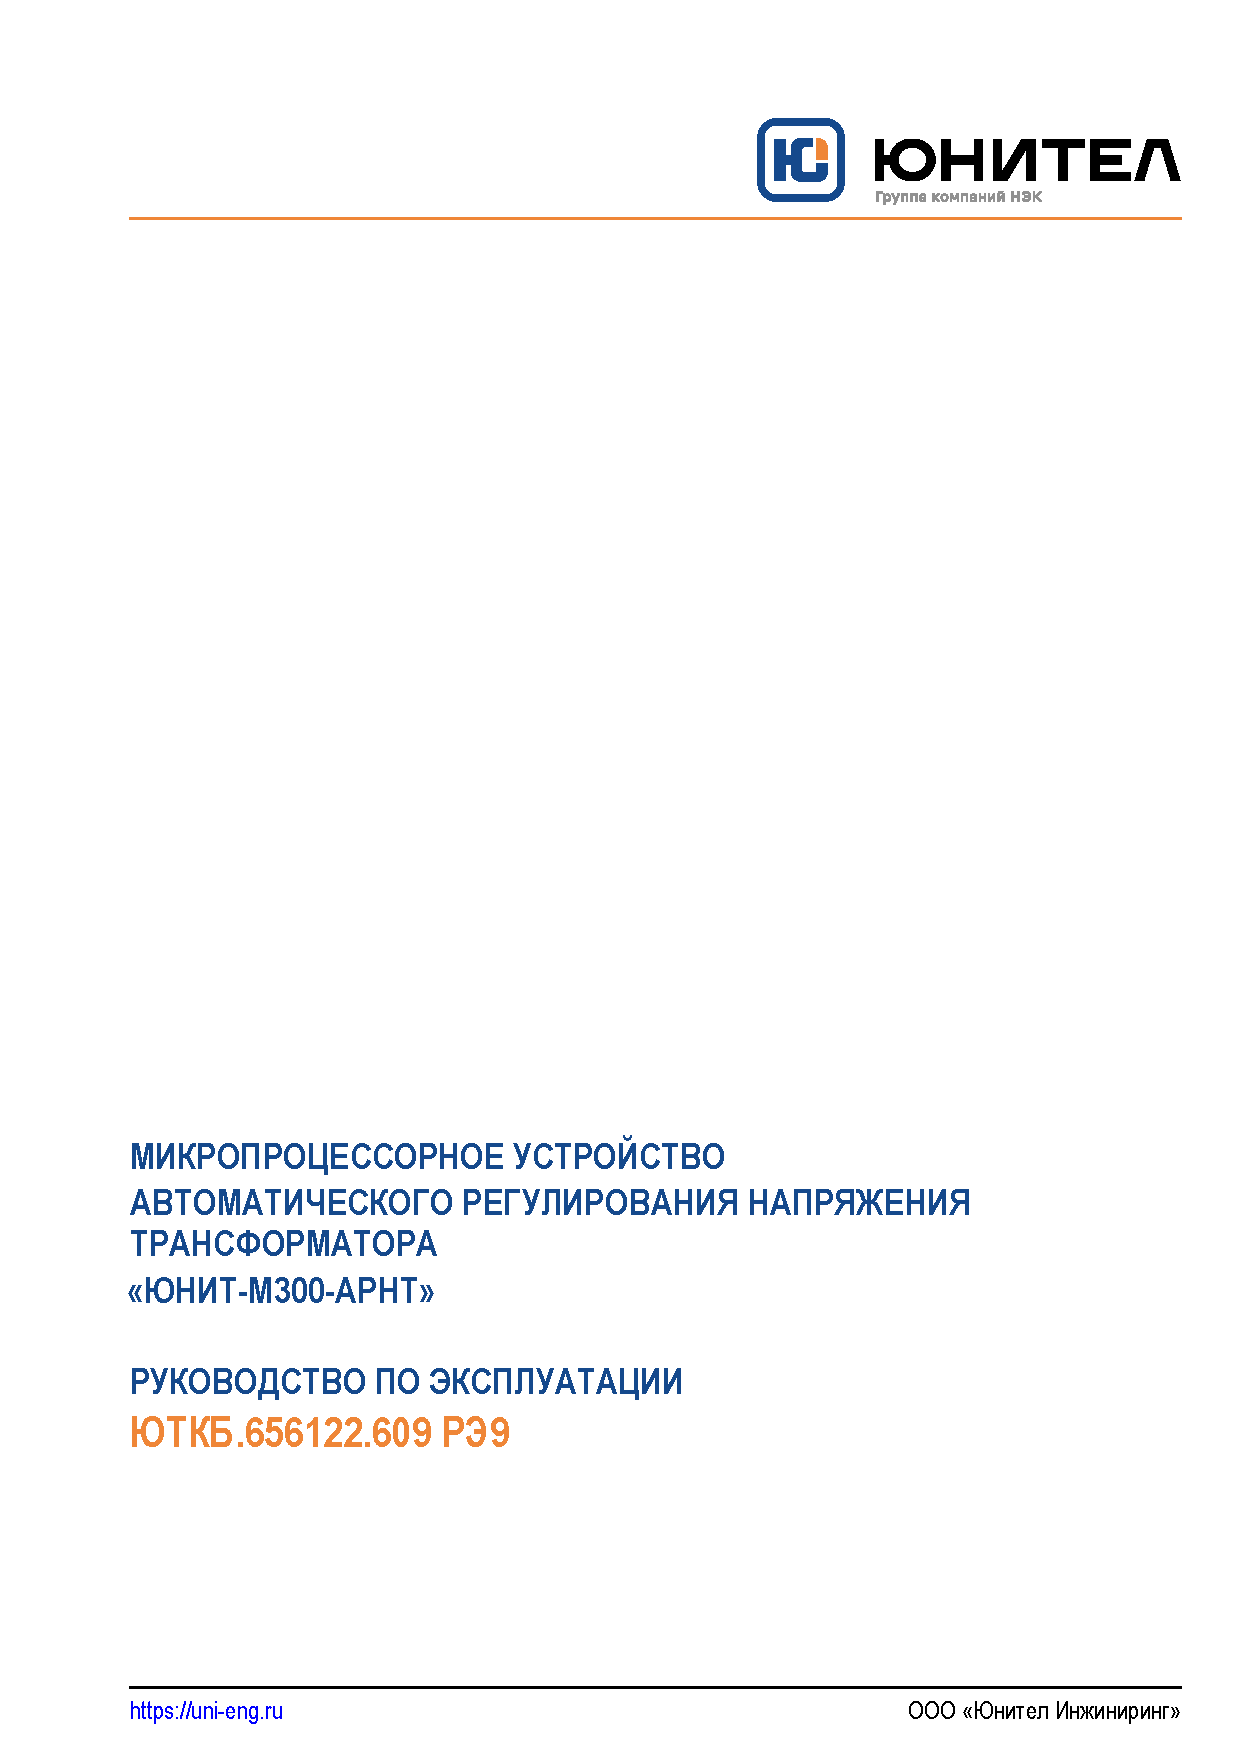
\includepdf[pages={1},width=0.5\textwidth, angle=90]{1.pdf} вставляем и поворачиваем pdf
%\begin{center}
%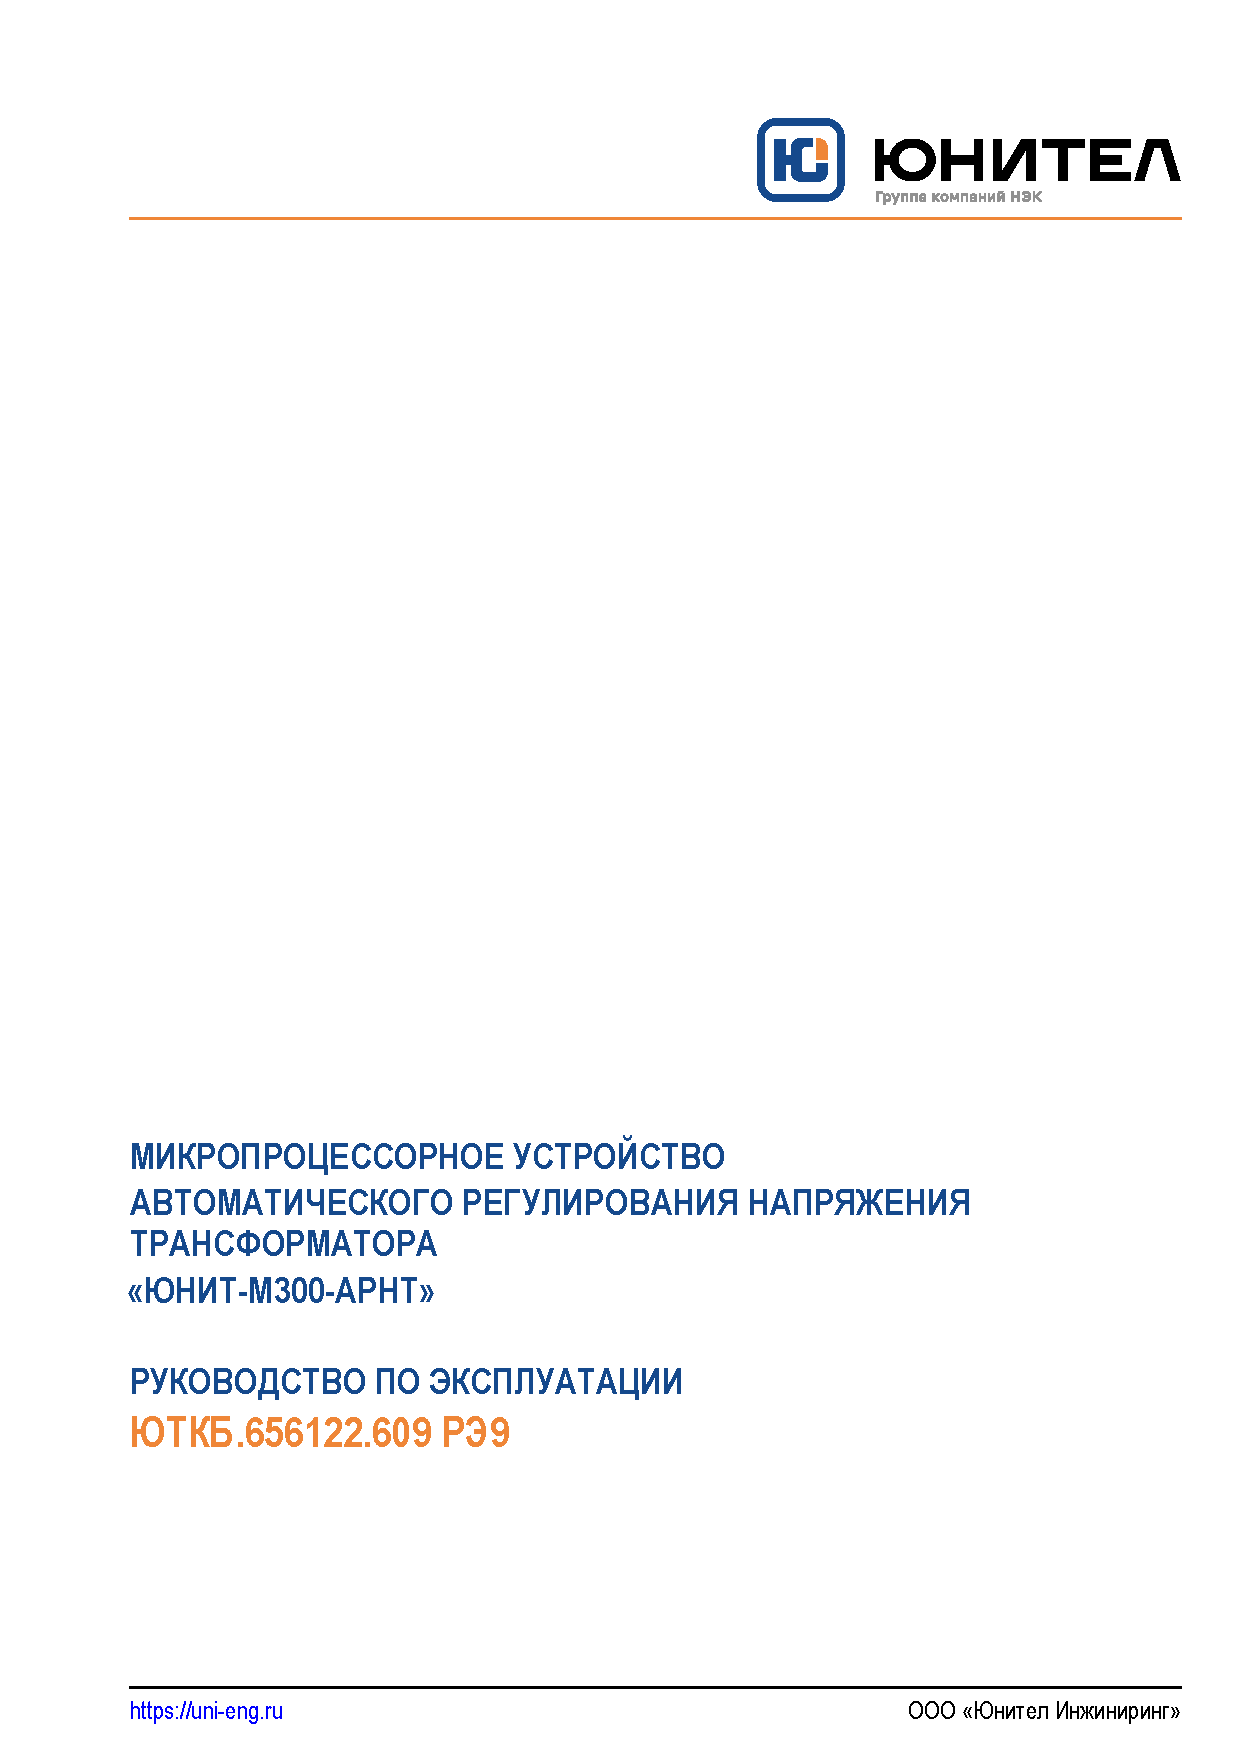
\includegraphics[width=1.4\textwidth]{1.pdf}
%\end{center}

\end{landscape}
\restoregeometry


